%-
% QUAN TRỌNG: Cần biên dịch bằng XeLaTeX hoặc LuaLaTeX
% Trong Overleaf: Settings → Compiler → chọn XeLaTeX
%-
% !TEX program = xelatex % (can also use "lualatex")
\documentclass[12pt,a4paper]{report}

% - Encoding & Font (XeLaTeX / LuaLaTeX) -
\usepackage{fontspec}
% Font mặc định (Latin Modern)

% - Tiếng Việt -
\usepackage{polyglossia}
\setdefaultlanguage{vietnamese}
\setotherlanguage{english}

% - Packages -
\usepackage{graphicx}
\usepackage{amsmath}
\usepackage{amssymb}
\usepackage{hyperref}
\usepackage{fancyhdr}
\usepackage{tabularx}
\usepackage{titlesec}
\usepackage{booktabs}
\usepackage{xcolor}
\usepackage{multirow}
\usepackage{makecell}
\usepackage{needspace}
\usepackage{etoolbox}
\usepackage{tikz}
\usepackage{tocloft}
\usepackage{float}
\usepackage{enumitem}
\usepackage{longtable}
\usepackage{cite}
\usepackage{listings}
\usepackage{subcaption}
\usepackage[nottoc]{tocbibind}
\usepackage{caption}
\usepackage{minted}
\usemintedstyle{friendly}
\usetikzlibrary{calc, shapes.geometric, arrows.meta, positioning, fit, backgrounds}


% - Geometry -
\usepackage[
    a4paper,
    left=2.5cm,
    right=2.5cm,
    top=2.5cm,
    bottom=3cm,
    footskip=1.5cm
]{geometry}

% - Màu sắc -
\definecolor{codegreen}{rgb}{0,0.6,0}
\definecolor{codegray}{rgb}{0.5,0.5,0.5}
\definecolor{codepurple}{rgb}{0.58,0,0.82}
\definecolor{backcolour}{rgb}{0.95,0.95,0.92}
\definecolor{borderblue}{RGB}{16,16,144}
\definecolor{mprimary}{HTML}{6C3FC0}
\definecolor{maccent}{HTML}{FF9F1C}
\definecolor{mgood}{HTML}{2EC4B6}

% - Code Python -
\lstdefinestyle{python}{
  language=Python,
  basicstyle=\ttfamily\footnotesize,
  keywordstyle=\bfseries\color{blue},
  commentstyle=\itshape\color{gray},
  stringstyle=\color{orange!70},
  numbers=left,
  numberstyle=\tiny\color{gray},
  backgroundcolor=\color{lightgray!20},
  breaklines=true,
  frame=single,
  showspaces=false,
  showstringspaces=false
}

% - Header/Footer -
\pagestyle{fancy}
\fancyhf{}
\renewcommand{\headrulewidth}{0.5pt}
\renewcommand{\footrulewidth}{0.5pt}
\fancyhead[C]{\textit{Phân tích dữ liệu thông minh - Nhóm SonicT2All}}
\fancyfoot[C]{\thepage}

% - Tiêu đề chương/mục -
\titleformat{\chapter}[display]
  {\centering\large\bfseries}{\chaptertitlename\ \thechapter}{10pt}{\large}
\titleformat{\section}
  {\normalfont\large\bfseries}{\thesection}{0.3em}{}
\titleformat{\subsection}
  {\normalfont\large\bfseries}{\thesubsection}{0.3em}{}

% - Mục lục -
\renewcommand{\contentsname}{\begin{center}\Large\bfseries MỤC LỤC\end{center}}
\setlength{\cftbeforetoctitleskip}{20pt}
\setlength{\cftaftertoctitleskip}{10pt}
\setlength{\cftparskip}{5pt}
\renewcommand{\numberline}[1]{\bfseries#1\hspace{0.5em}}
\setcounter{secnumdepth}{3}

\begin{document}
\sloppy

% ============================================================
% TRANG BÌA
% ============================================================
\thispagestyle{empty}
\begin{tikzpicture}[remember picture, overlay]
  \draw[borderblue, line width=1pt]
    ([shift={(1cm,1cm)}]current page.south west) rectangle
    ([shift={(-1cm,-1cm)}]current page.north east);
  \draw[borderblue, line width=1pt]
    ([shift={(1.1cm,1.1cm)}]current page.south west) rectangle
    ([shift={(-1.1cm,-1.1cm)}]current page.north east);
\end{tikzpicture}

\begin{center}
    \vspace*{0cm}
    {\large BỘ GIÁO DỤC VÀ ĐÀO TẠO \par}
    \vspace{0.3cm}
    {\large TRƯỜNG ĐẠI HỌC KHOA HỌC TỰ NHIÊN \par}
    \vspace{0.3cm}
    {\large KHOA CÔNG NGHỆ THÔNG TIN \par}
    \vspace{0.3cm}
    {\large\textbf{PHÂN TÍCH DỮ LIỆU THÔNG MINH} \par}
    \vspace{0.3cm}

    \begin{center}
        
\includegraphics[width=6cm]{LogoTruong.png}
    \end{center}
    \vspace{0.3cm}

    {\large\textbf{BÁO CÁO MÔN HỌC} \par}
    \vspace{0.3cm}
    {\large\textbf{PROJECT - WORLD MUSIC INTELLIGENCE MONITOR} \par}
    \vspace{0.5cm}

    \begin{tabular}{lll}
        \textbf{Giảng viên hướng dẫn} & : & TS. Nguyễn Tiến Huy \\
                                       & & TS. Lê Thanh Tùng \\
                                       & & ThS. Nguyễn Thanh Tình \\
                                       & & \\
        \textbf{Nhóm thực hiện}        & : & SonicT2All \\
                                       & & \\
        \textbf{Lớp}                   & : & CQ2023 \\
                                       & & \\
        \textbf{Nhóm sinh viên thực hiện} & : & \\
        & & Bàng Mỹ Linh \hspace{1.5cm}     | 23122009 \\
        & & Lại Nguyễn Hồng Thanh \hspace{0.45cm} | 23122018 \\
        & & Phan Huỳnh Châu Thịnh \hspace{0.45cm} | 23122019 \\
        & & Nguyễn Gia Bảo \hspace{1.1cm}   | 23122015 \\
        & & Nguyễn Ngọc Như Quỳnh \hspace{0.4cm} | 23120080 \\
    \end{tabular}

    \vfill
    {\Large\textbf{Tháng 6 năm 2026} \par}
\end{center}
\clearpage

% ============================================================
% MỤC LỤC & DANH MỤC
% ============================================================
\tableofcontents
\clearpage
\listoftables
\clearpage
\listoffigures
\clearpage

% ============================================================
% DANH MỤC VIẾT TẮT
% ============================================================
\chapter*{DANH MỤC VIẾT TẮT}
\addcontentsline{toc}{chapter}{DANH MỤC VIẾT TẮT}

\begin{tabularx}{\textwidth}{lX}
\textbf{API} & Application Programming Interface - Giao diện lập trình ứng dụng \\
\textbf{CORS} & Cross-Origin Resource Sharing - Chia sẻ tài nguyên giữa các nguồn gốc \\
\textbf{EDA} & Exploratory Data Analysis - Phân tích dữ liệu khám phá \\
\textbf{JWT} & JSON Web Token - Mã thông báo web JSON \\
\textbf{MIS} & Music Intelligence Score - Điểm thông minh âm nhạc \\
\textbf{ML} & Machine Learning - Học máy \\
\textbf{MV} & Music Video - Video ca nhạc \\
\textbf{NLP} & Natural Language Processing - Xử lý ngôn ngữ tự nhiên \\
\textbf{PCA} & Principal Component Analysis - Phân tích thành phần chính \\
\textbf{RBAC} & Role-Based Access Control - Kiểm soát truy cập theo vai trò \\
\textbf{REST} & Representational State Transfer - Kiểu kiến trúc API \\
\textbf{SHAP} & SHapley Additive exPlanations - Phương pháp giải thích mô hình \\
\textbf{SSE} & Server-Sent Events - Sự kiện gửi từ máy chủ \\
\textbf{SSO} & Single Sign-On - Đăng nhập một lần \\
\textbf{VADER} & Valence Aware Dictionary and sEntiment Reasoner - Công cụ phân tích cảm xúc \\
\textbf{WCSS} & Within-Cluster Sum of Squares - Tổng bình phương trong cụm \\
\end{tabularx}
\clearpage

% ============================================================
% CHƯƠNG 1 — PHÂN CÔNG CÔNG VIỆC
% ============================================================
\chapter{PHÂN CÔNG CÔNG VIỆC}

Dự án \textbf{World Music Intelligence Monitor} được thực hiện trong khoảng \textbf{5 tuần}, với công việc được phân chia theo vai trò kỹ thuật chuyên biệt. Tất cả thành viên đều tham gia vào quá trình thu thập, xử lý và phân tích dữ liệu.

\begin{tabularx}{\textwidth}{|c|l|X|c|}
\hline
\textbf{MSSV} & \textbf{Họ tên} & \textbf{Nội dung đảm nhiệm} & \textbf{Hoàn thành} \\
\hline
23122009 & Bàng Mỹ Linh &
    \textbf{Frontend + Data Visualization:} Xây dựng giao diện Next.js (Dashboard, World Map, Trend page, Prediction page); thiết kế các biểu đồ trực quan hoá (Donut chart, Heatmap, KPI cards, Radar chart, Bar chart) bằng Recharts; hỗ trợ phân tích phân phối dữ liệu âm nhạc
    & 100\% \\
\hline
23122019 & Phan Huỳnh Châu Thịnh &
    \textbf{AI Engineering + Thu thập \& Xử lý dữ liệu:} Xây dựng mô hình XGBoost dự đoán hit trên Kaggle; thiết kế pipeline đặc trưng đa nguồn; phát triển module phân cụm K-Means; cài đặt VADER Sentiment; xây dựng ReAct Agent với Gemini AI; crawl và chuẩn hoá dữ liệu từ Last.fm, YouTube, Reddit, Deezer
    & 100\% \\
\hline
23122018 & Lại Nguyễn Hồng Thanh &
    \textbf{QA + Testing:} Kiểm thử các API endpoint (unit test, integration test); kiểm tra luồng dữ liệu; test model dự đoán; test bảo mật Clerk; hỗ trợ phân tích dữ liệu và viết báo cáo
    & 100\% \\
\hline
23122015 & Nguyễn Gia Bảo &
    \textbf{Backend:} Xây dựng toàn bộ hệ thống FastAPI (routers, services, scheduler APScheduler); tích hợp Firebase Firestore làm database; thiết kế cache 3 lớp; triển khai trên Render.com; hỗ trợ phân tích dữ liệu
    & 100\% \\
\hline
23120080 & Nguyễn Ngọc Như Quỳnh &
    \textbf{API + Bảo mật + Database:} Tích hợp các API ngoài (YouTube Data API, Reddit API, Last.fm API, Deezer API, Gemini AI API); thiết lập xác thực người dùng với Clerk; thiết kế schema Firestore; quản lý .env và API key; hỗ trợ phân tích dữ liệu
    & 100\% \\
\hline
\end{tabularx}

% ============================================================
% CHƯƠNG 2 — TỔNG QUAN DỰ ÁN
% ============================================================
\chapter{TỔNG QUAN DỰ ÁN}

\section{Giới thiệu bài toán}

Ngành công nghiệp âm nhạc toàn cầu đang đối mặt với nhiều thách thức trong việc theo dõi dữ liệu:
\begin{itemize}[leftmargin=*]
    \item \textbf{Phân mảnh dữ liệu:} Thông tin nghe nhạc rải rác trên hàng chục nền tảng, thiếu một hệ thống tổng hợp để tạo bức tranh toàn cảnh.
    \item \textbf{Độ trễ cao:} Các bảng xếp hạng truyền thống cập nhật chậm, không phản ánh kịp thời xu hướng viral trên mạng xã hội.
    \item \textbf{Thiếu chiều sâu phân tích:} Biết một bài hát đang "hot" nhưng không hiểu rõ \textit{tại sao} nó hot.
\end{itemize}

Dự án \textbf{World Music Intelligence Monitor} giải quyết các vấn đề trên thông qua:
\begin{enumerate}[leftmargin=*]
    \item \textbf{Tổng hợp đa nguồn:} Gom dữ liệu từ YouTube, Last.fm, Reddit, Deezer vào một dashboard theo thời gian thực.
    \item \textbf{Cập nhật liên tục:} Áp dụng pipeline polling 6h kết hợp cache để dữ liệu luôn phản ánh đúng xu hướng.
    \item \textbf{Phân tích chuyên sâu bằng AI:} Tích hợp AI (Gemini, XGBoost, K-Means, VADER) để giải thích nguyên nhân viral, dự đoán hit và phân tích thị hiếu quốc gia.
\end{enumerate}

\section{Các hệ thống liên quan}

Một số nền tảng phân tích âm nhạc hiện có trên thị trường:
\begin{itemize}
    \item \textbf{Chartmetric:} Nền tảng analytics thương mại, tổng hợp dữ liệu từ Spotify, Apple Music, YouTube, TikTok, Shazam. Tuy nhiên, phí sử dụng cao (từ \$160/tháng) và không cung cấp khả năng phân cụm thị hiếu theo quốc gia hay AI agent hỏi đáp.
    \item \textbf{Soundcharts:} Tương tự Chartmetric, tập trung vào theo dõi playlist và radio airplay. Thiếu tính năng phân tích cảm xúc cộng đồng (social sentiment) và dự đoán hit.
    \item \textbf{Spotify for Artists:} Miễn phí nhưng giới hạn trong hệ sinh thái Spotify, không tổng hợp đa nguồn và không có AI insights.
\end{itemize}

\noindent
\textbf{Điểm khác biệt} của hệ thống Music Monitor: (1) Hoàn toàn miễn phí và mã nguồn mở; (2) Tổng hợp đa nguồn API không phụ thuộc vào một nền tảng duy nhất; (3) Phân cụm K-Means theo quốc gia - tính năng chưa có trên các nền tảng thương mại; (4) AI Agent (ReAct) cho phép hỏi đáp tự nhiên về dữ liệu; (5) Hit prediction với Explainable AI.

\section{Mục tiêu hệ thống}

\begin{itemize}
    \item \textbf{Mục tiêu 1:} Xây dựng hệ thống thu thập dữ liệu thời gian thực từ đa nguồn âm nhạc toàn cầu.
    \item \textbf{Mục tiêu 2:} Phân tích và trực quan hoá xu hướng âm nhạc theo nhiều chiều (thể loại, quốc gia, cảm xúc, độ viral).
    \item \textbf{Mục tiêu 3:} Ứng dụng Machine Learning để dự đoán khả năng trở thành bản hit của một bài hát.
    \item \textbf{Mục tiêu 4:} Phân cụm thị hiếu âm nhạc theo quốc gia sử dụng K-Means + PCA.
    \item \textbf{Mục tiêu 5:} Triển khai AI Agent (ReAct) cho phép người dùng hỏi đáp thông minh về âm nhạc.
\end{itemize}

\section{Kiến trúc hệ thống tổng quan}

Hệ thống được xây dựng theo kiến trúc \textbf{3-tier} rõ ràng:

\begin{itemize}
    \item \textbf{Tầng Frontend (Next.js 14):} Giao diện người dùng sử dụng App Router, TypeScript, TailwindCSS. Trực quan hoá dữ liệu bằng Recharts (bar, line, radar, donut chart). Hiệu ứng animation với Framer Motion. Quản lý state với SWR (stale-while-revalidate). Hỗ trợ dark/light mode qua next-themes. Triển khai trên Vercel, cổng 3000.
    \item \textbf{Tầng Backend (FastAPI + Python 3.11):} Xử lý logic nghiệp vụ, điều phối AI/ML, lên lịch thu thập dữ liệu. Triển khai trên Render.com, cổng 8000.
    \item \textbf{Tầng Data (Firebase Firestore + File Cache):} Lưu trữ và cache dữ liệu đã thu thập.
\end{itemize}

\noindent
Frontend giao tiếp với Backend qua \textbf{HTTP REST + SSE (Server-Sent Events)} cho streaming real-time. Backend tương tác với các nguồn bên ngoài (Last.fm, YouTube, Reddit, Deezer) và các mô hình AI (Gemini, XGBoost, K-Means).

\begin{figure}[H]
    \centering
    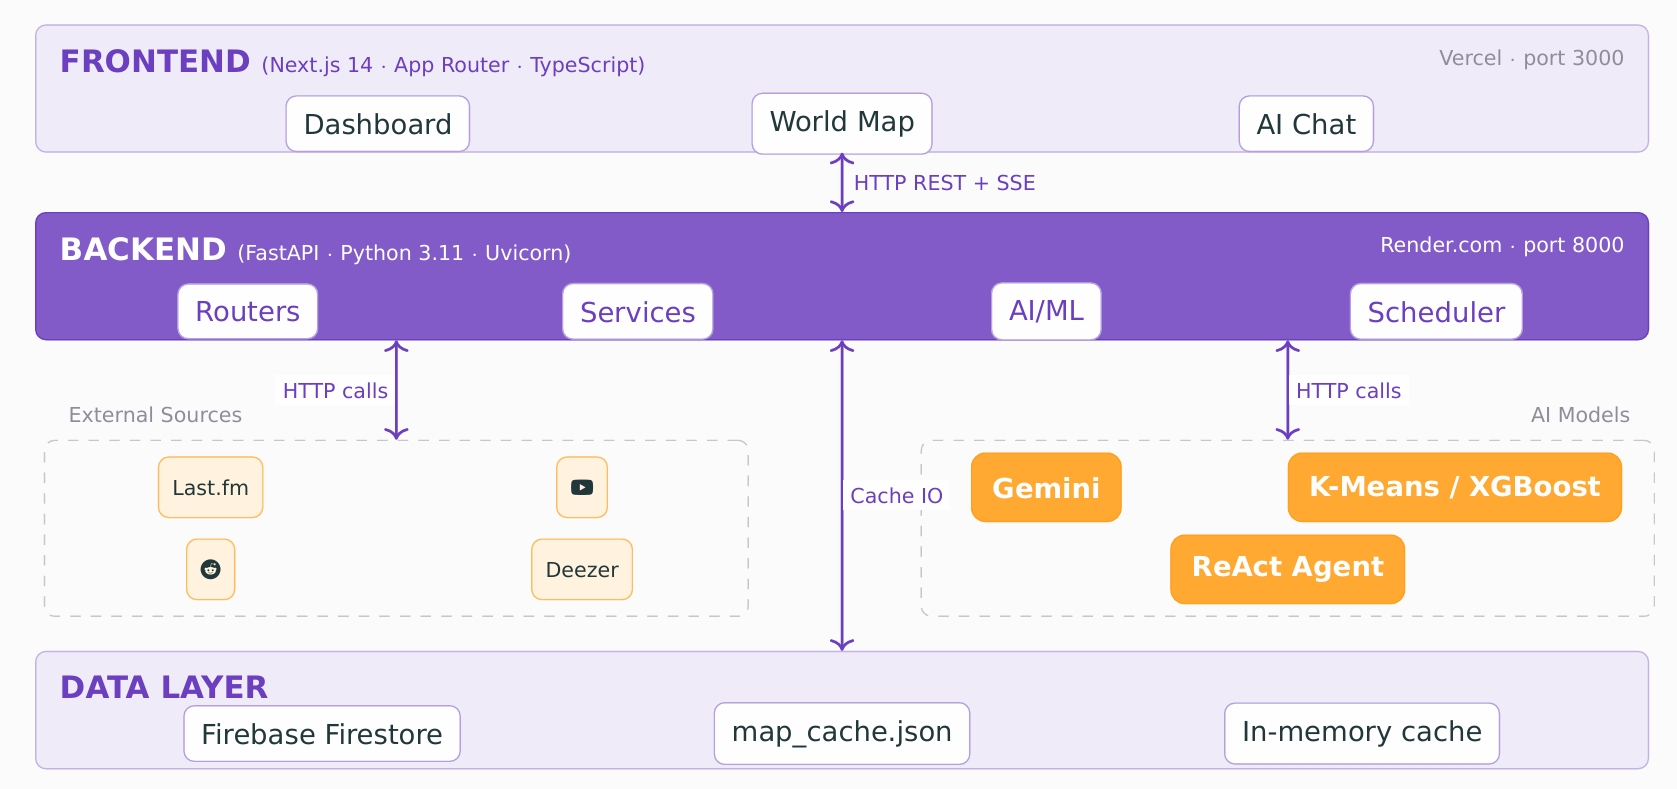
\includegraphics[width=\textwidth]{figures/system-architecture.jpeg}
    \caption{Kiến trúc hệ thống 3-tier: Frontend (Next.js) - Backend (FastAPI) - Data Layer (Firestore + Cache)}
    \label{fig:architecture}
\end{figure}

\section{Nguồn dữ liệu}

Hệ thống tích hợp \textbf{4 nguồn dữ liệu thu thập} chính, kết hợp với \textbf{Gemini AI} (Google) làm lớp xử lý ngôn ngữ tự nhiên:


\begin{table}[H]
\centering
\caption{Tổng quan các nguồn dữ liệu tích hợp}
\label{tab:data_sources}
\begin{tabularx}{\textwidth}{|l|l|X|l|}
\hline
\textbf{Nguồn} & \textbf{API/Phương thức} & \textbf{Dữ liệu cung cấp} & \textbf{Chế độ thu thập} \\
\hline
Last.fm & REST API (key) & Top charts toàn cầu/quốc gia, playcount, listeners & Polling 6h \\
\hline
YouTube Data API v3 & REST API (OAuth key) & Views, likes, comments, growth stats & On-demand \\
\hline
Reddit & Public JSON API & Hot posts, upvotes, số bình luận & On-demand \\
\hline
Deezer & REST API (không cần key) & Chart quốc gia, TikTok viral playlist, metadata, preview 30s & On-demand \\
\hline
\end{tabularx}
\end{table}

Hệ thống lựa chọn Deezer làm nguồn dữ liệu chính cho bản đồ World Map vì các lý do sau:

\begin{itemize}[leftmargin=*]
    \item \textbf{Ưu điểm của Deezer API:} Cung cấp endpoint \texttt{/editorial/\{country\_id\}/charts} hoàn toàn miễn phí, không cần API key. (Ngược lại, Spotify yêu cầu tài khoản Premium để truy xuất Editorial playlists\footnote{Hệ thống có module \texttt{services/spotify.py} hỗ trợ Spotify Web API, tuy nhiên do giới hạn Premium nên Spotify không được sử dụng làm nguồn chính mà chỉ cung cấp New Releases bổ trợ.}).
    \item \textbf{Hạn chế dữ liệu:} Kho nhạc bản quyền của Deezer tại một số quốc gia (như Việt Nam - ID 122) không đầy đủ, dẫn đến bảng xếp hạng bị nhiễu (VD: xuất hiện nhiều nhạc Ấn Độ, Latin).
    \item \textbf{Giải pháp Local Genre Boost:} Bổ sung thủ công các tag thể loại đặc trưng địa phương (v-pop, ballad, rap cho VN; k-pop cho Hàn Quốc...) trước khi chạy K-Means clustering.
    \item \textbf{Tính chính xác của AI Insights:} Dù dữ liệu gốc có nhiễu, AI phân tích vẫn sát thực tế. Nguyên nhân là K-Means phân cụm dựa trên vector đặc trưng thể loại (không phụ thuộc hoàn toàn vào chart thô), và Gemini phân tích văn hoá từ nguồn fallback \texttt{geo.getTopTracks} của Last.fm.
\end{itemize}

% ============================================================
% CHƯƠNG 3 — THU THẬP VÀ XỬ LÝ DỮ LIỆU
% ============================================================
\chapter{THU THẬP VÀ XỬ LÝ DỮ LIỆU}

\section{Pipeline thu thập dữ liệu}

\subsection{Cơ chế Scheduler}

Backend sử dụng \textbf{APScheduler} (AsyncIO Scheduler) để tự động hoá việc thu thập dữ liệu. Do các nền tảng âm nhạc (Youtube, Last.fm, Deezer) không cung cấp webhook nên việc sử dụng polling định kỳ là lựa chọn thực tế nhất khi kết hợp cache.

\begin{itemize}
    \item \textbf{Polling 6h:} Last.fm global top tracks được cập nhật mỗi 6 tiếng, ghi vào Firestore collection \texttt{cache/global\_top} và lưu lịch sử vào \texttt{historical\_charts/\allowbreak{}global\_top/history}. Khoảng thời gian 6h được chọn để tối ưu quota Firebase free tier (50.000 lượt đọc/ngày, 20.000 lượt ghi/ngày).
    \item \textbf{On-demand:} YouTube stats, Reddit posts, Deezer chart được fetch khi người dùng yêu cầu, sử dụng \texttt{asyncio.gather()} để song song hoá.
\end{itemize}

Sơ đồ luồng hoạt động của cơ chế lập lịch (Scheduler) định kỳ và yêu cầu dữ liệu tức thì (On-demand) được thể hiện ở Hình~\ref{fig:scheduler_flow}.

\begin{figure}[H]
    \centering
    \resizebox{\textwidth}{!}{
    \begin{tikzpicture}[
        node distance = 1.0cm and 0.8cm,
        box/.style = {draw, rectangle, rounded corners=5pt, minimum width=3.0cm, minimum height=1.1cm, align=center, font=\small\bfseries, line width=1pt},
        trigger/.style = {box, fill=mprimary!8, draw=mprimary},
        process/.style = {box, fill=borderblue!6, draw=borderblue},
        database/.style = {box, rounded corners=10pt, fill=mgood!8, draw=mgood},
        api/.style = {box, fill=maccent!8, draw=maccent},
        arrow/.style = {draw=black!70, -{Stealth[scale=1.1]}, line width=1.1pt},
        container/.style = {draw=black!40, dashed, rounded corners=8pt, line width=0.8pt, fill=black!2}
    ]

        % === Left Flow: Polling (6h) ===
        \node (trigger6h) [trigger] {IntervalTrigger\\(Mỗi 6 giờ)};
        
        \node (scheduler) [process, below=of trigger6h] {APScheduler\\(FastAPI Background)};
        
        \node (pollJobs) [process, below=of scheduler] {Jobs:\\poll\_lastfm\_charts()\\poll\_youtube\_stats()};
        
        \node (extAPIs) [api, left=of pollJobs, xshift=-0.5cm] {External APIs\\(Last.fm, YouTube)};
        
        \node (firestore) [database, below=of pollJobs, yshift=-0.2cm] {Firestore DB\\cache/global\_top\\history};

        % === Right Flow: On-Demand ===
        \node (userReq) [trigger, right=of trigger6h, xshift=1.5cm] {User Request\\(Yêu cầu Frontend)};
        
        \node (fastapiEP) [process, below=of userReq] {FastAPI Endpoint\\(On-demand route)};
        
        \node (gather) [process, below=of fastapiEP] {asyncio.gather()\\(Song song hóa)};
        
        \node (onDemandAPIs) [api, right=of gather, xshift=0.5cm] {External APIs\\(YouTube, Reddit,\\Deezer)};
        
        \node (frontend) [process, below=of gather, yshift=-0.4cm] {Frontend UI\\(Next.js Dashboard)};

        % === Arrows ===
        % Polling
        \draw [arrow] (trigger6h) -- (scheduler);
        \draw [arrow] (scheduler) -- (pollJobs);
        \draw [arrow, <->] (pollJobs) -- (extAPIs);
        \draw [arrow] (pollJobs) -- (firestore);

        % On-Demand
        \draw [arrow] (userReq) -- (fastapiEP);
        \draw [arrow] (fastapiEP) -- (gather);
        \draw [arrow, <->] (gather) -- (onDemandAPIs);
        \draw [arrow] (gather) -- (frontend);

        % Containers (Fit backgrounds)
        \begin{scope}[on background layer]
            \node[container, fit=(trigger6h) (pollJobs) (extAPIs) (firestore), label={[font=\sffamily\bfseries\color{borderblue}]above:Cơ chế Polling Định kỳ (Background)}] (boxPolling) {};
            \node[container, fit=(userReq) (gather) (onDemandAPIs) (frontend), label={[font=\sffamily\bfseries\color{borderblue}]above:Cơ chế On-Demand (Real-time)}] (boxOnDemand) {};
        \end{scope}

    \end{tikzpicture}
    }
    \caption{Sơ đồ cơ chế hoạt động của Scheduler (APScheduler) và Luồng Yêu cầu On-demand}
    \label{fig:scheduler_flow}
\end{figure}


\subsection{Cache 3 lớp}
Vì hệ thống cần gọi các API và sẽ dễ gặp tình trạng hết quota. Vì vậy, để đảm bảo hiệu suất và không vượt quota, hệ thống áp dụng \textbf{cache 3 lớp}:
\begin{enumerate}
    \item \textbf{Firestore (Cloud):} Lưu trữ dữ liệu chart mới nhất + lịch sử time-series YouTube. Đây là nguồn dữ liệu xác minh tính chân thật cho frontend.
    \item \textbf{map\_cache.json (File):} Cache kết quả clustering K-Means World Map. Tính toán K-Means lần đầu mất 60-90 giây (cào 89 quốc gia); cache file giúp lần sau tải tức thì. File bị xoá khi có yêu cầu refresh.
    \item \textbf{In-memory (RAM):} Cache Gemini AI insights theo ngày. Mỗi AI Insight (country insight, daily briefing, trend explanation) chỉ gọi Gemini 1 lần/ngày để không vượt quota free tier 14 req/phút.
\end{enumerate}

\subsection{Xử lý dữ liệu từ các nguồn}

Hệ thống xử lý đặc thù cho từng nguồn dữ liệu như sau:

\begin{itemize}[leftmargin=*]
    \item \textbf{Last.fm:}
    \begin{itemize}
        \item \textit{API sử dụng:} \texttt{chart.getTopTracks} và \texttt{geo.getTopTracks}.
        \item \textit{Dữ liệu thu thập:} \texttt{playcount} (tổng lượt nghe) và \texttt{listeners} (số người nghe độc lập).
        \item \textit{Vai trò:} Phản ánh sức sống dài hạn nhờ cơ chế "scrobbling". Dữ liệu này làm thước đo nền tảng (baseline) để tính điểm MIS (Music Intelligence Score).
        \item \textit{Tiền xử lý:} Chuẩn hoá văn bản (xoá HTML entities, unicode), chuyển đổi sang số nguyên (int).
    \end{itemize}

    \item \textbf{YouTube Data API v3:}
    \begin{itemize}
        \item \textit{Phương thức:} Tìm kiếm MV qua query \texttt{"\{track\} \{artist\} official music video"} $\rightarrow$ fetch stats.
        \item \textit{Dữ liệu thu thập:} \texttt{views} (độ phủ sóng), \texttt{likes} và \texttt{comments} (tương tác chủ động).
        \item \textit{Vai trò:} Là đầu vào trọng tâm tính Viral Score (xem công thức~\eqref{eq:viral_score}) và phát hiện sự bất thường (spike).
        \item \textit{Xử lý đặc thù:} Áp dụng \textbf{decay factor} (hệ số suy giảm) theo tuổi MV để tránh các bài hát cũ bị tính điểm viral không thực tế.
    \end{itemize}

    \item \textbf{Reddit:}
    \begin{itemize}
        \item \textit{Phương thức:} Gọi API \texttt{r/\{sub\}/hot.json} (kèm User-Agent để tránh block).
        \item \textit{Dữ liệu thu thập:} \texttt{title} (ngữ cảnh), \texttt{score} (upvotes), và \texttt{num\_comments}.
        \item \textit{Vai trò:} Đóng góp 30\% vào Viral Score và làm nguyên liệu văn bản cho AI phân tích cảm xúc (chỉ lấy bài trong 24h).
    \end{itemize}

    \item \textbf{Deezer:}
    \begin{itemize}
        \item \textit{Phương thức:} Gọi API miễn phí \texttt{/editorial/\{id\}/\allowbreak{}charts} và \texttt{/playlist/\{id\}/\allowbreak{}tracks}.
        \item \textit{Dữ liệu thu thập:} Chart quốc gia (strict mode), TikTok Viral, preview audio 30s, ảnh cover, BPM.
        \item \textit{Vai trò:} Phục vụ phân cụm K-Means cho World Map và làm giàu dữ liệu hiển thị trên Dashboard.
    \end{itemize}
\end{itemize}

Sơ đồ thuật toán tính toán Decay Factor theo độ tuổi MV được trình bày ở Hình~\ref{fig:decay_factor}.

\begin{figure}[H]
    \centering
    \resizebox{0.85\textwidth}{!}{
    \begin{tikzpicture}[
        node distance = 0.6cm and 1.5cm,
        box/.style = {draw, rectangle, rounded corners=5pt, minimum width=2.5cm, minimum height=0.9cm, align=center, font=\small\bfseries, line width=1pt},
        decision/.style = {draw, diamond, aspect=2.2, minimum width=3.2cm, minimum height=0.9cm, align=center, font=\small\bfseries, line width=1pt, fill=maccent!10, draw=maccent},
        process/.style = {box, fill=borderblue!6, draw=borderblue},
        input/.style = {box, fill=mgood!10, draw=mgood},
        arrow/.style = {draw=black!70, -{Stealth[scale=1.1]}, line width=1.1pt}
    ]

        % Input
        \node (input) [input] {Input:\\\texttt{days\_old}};
        
        % Decisions
        \node (cond365) [decision, below=0.8cm of input] {$> 365$ ngày?};
        \node (cond100) [decision, below=0.6cm of cond365] {$> 100$ ngày?};
        \node (cond30)  [decision, below=0.6cm of cond100] {$> 30$ ngày?};
        
        % Factors
        \node (fact365) [process, right=of cond365] {decay\_factor = 0.02};
        \node (fact100) [process, right=of cond100] {decay\_factor = 0.15};
        \node (fact30)  [process, right=of cond30] {decay\_factor = 0.50};
        \node (fact0)   [process, below=0.6cm of cond30] {decay\_factor = 1.00};
        
        % Compute
        \node (compute) [input, right=of fact100, xshift=1.0cm] {Tính toán:\\\texttt{mock\_growth\_24h =}\\\texttt{min(base\_growth * decay, 600)}};

        % Arrows
        \draw [arrow] (input) -- (cond365);
        \draw [arrow] (cond365) -- node[anchor=east, font=\footnotesize\bfseries] {Sai} (cond100);
        \draw [arrow] (cond100) -- node[anchor=east, font=\footnotesize\bfseries] {Sai} (cond30);
        \draw [arrow] (cond30) -- node[anchor=east, font=\footnotesize\bfseries] {Sai} (fact0);
        
        \draw [arrow] (cond365) -- node[anchor=south, font=\footnotesize\bfseries] {Đúng} (fact365);
        \draw [arrow] (cond100) -- node[anchor=south, font=\footnotesize\bfseries] {Đúng} (fact100);
        \draw [arrow] (cond30) -- node[anchor=south, font=\footnotesize\bfseries] {Đúng} (fact30);
        
        % Connect to compute
        \coordinate (c1) at ($(fact100.east) + (0.6cm,0)$);
        
        \draw [arrow] (fact365.east) -| (c1) |- (compute.west);
        \draw [arrow] (fact100.east) -- (compute.west);
        \draw [arrow] (fact30.east) -| (c1) |- (compute.west);
        \draw [arrow] (fact0.east) -| (c1) |- (compute.west);

    \end{tikzpicture}
    }
    \caption{Lưu đồ xử lý Decay Factor theo độ tuổi MV YouTube}
    \label{fig:decay_factor}
\end{figure}

Các mốc thời gian và hệ số decay được thiết kế dựa trên quan sát vòng đời thực tế của một MV trên YouTube:
\begin{itemize}
    \item \textbf{0 - 30 ngày ($decay = 1.0$):} Giai đoạn phát hành, lượt xem phản ánh đúng sức hút thực tế.
    \item \textbf{30 - 100 ngày ($decay = 0.5$):} Qua đỉnh quảng bá, độ hot bắt đầu giảm nhiệt.
    \item \textbf{100 - 365 ngày ($decay = 0.15$):} Giai đoạn ``long tail'', lượt xem chủ yếu đến từ thuật toán đề xuất, ít phản ánh xu hướng mới.
    \item \textbf{$> 365$ ngày ($decay = 0.02$):} Bài hát cũ, gần như triệt tiêu điểm viral để nhường chỗ cho bài mới.
\end{itemize}

Công thức tính tốc độ tăng trưởng giả lập trong 24 giờ:
\begin{equation}
\texttt{mock\_growth\_24h} = \min(\texttt{base\_growth} \times \texttt{decay\_factor},\; 600)
\label{eq:mock_growth}
\end{equation}

\begin{itemize}
    \item \textbf{\texttt{base\_growth}:} Ước tính bằng $\min(\texttt{views} / 1{,}000{,}000 \times 12,\; 600)$, mô phỏng đà tăng trưởng tự nhiên.
    \item \textbf{Ngưỡng tối đa 600\%:} Ngăn chặn điểm số phi thực tế từ các MV siêu viral (hàng tỷ view), giữ điểm số trong phạm vi hợp lý.
\end{itemize}

\section{Xử lý dữ liệu cho World Map}

World Map là chức năng phức tạp nhất về xử lý dữ liệu. Quy trình gồm 3 bước:

\begin{enumerate}[leftmargin=*]
    \item \textbf{Bước 1 - Xây dựng vector đặc trưng genre:} 
    \begin{itemize}
        \item Truy xuất bảng xếp hạng của 89 quốc gia qua Deezer API (lấy top 10 bài).
        \item Gọi Last.fm \texttt{artist.getTopTags} để lấy \textbf{genre tags} (thể loại âm nhạc do người dùng dán).
        \item Fallback sang \texttt{geo.getTopTracks} nếu Deezer trả về thiếu tag. 
        \item Bổ sung \textbf{Local Genre Boost} thủ công cho các quốc gia có nhạc địa phương đặc thù (VD: v-pop, k-pop, bollywood).
    \end{itemize}

    \item \textbf{Bước 2 - K-Means Clustering \& PCA:} 
    \begin{itemize}
        \item Xây dựng \textbf{vector 16 chiều} dựa trên 16 thể loại chuẩn (pop, hip-hop, k-pop, rock,...).
        \item Chạy thuật toán \textbf{K-Means} với $k=6$ cụm (chọn qua phương pháp Elbow), tương ứng với 6 vùng văn hoá âm nhạc chính.
        \item Áp dụng \textbf{PCA 2 chiều} (Phân tích thành phần chính) để giảm từ không gian 16 chiều xuống 2 trục tọa độ $(x, y)$, giúp trực quan hóa phân cụm dễ dàng trên bản đồ 2D.
    \end{itemize}

    \item \textbf{Bước 3 - Gán nhãn cụm:} 
    \begin{itemize}
        \item Tự động đặt tên cụm dựa trên thể loại nổi bật nhất của cụm (\texttt{genre\_means.\allowbreak{}idxmax()}). VD: ``K-POP-dominant''.
    \end{itemize}
\end{enumerate}

Sơ đồ quy trình phân cụm và giảm chiều dữ liệu được minh hoạ chi tiết ở Hình~\ref{fig:kmeans_pca}.

\begin{figure}[H]
    \centering
    \resizebox{0.9\textwidth}{!}{
    \begin{tikzpicture}[
        node distance = 1.0cm and 1.5cm,
        shadow/.style={preaction={fill=black, opacity=0.15, transform canvas={xshift=3pt, yshift=-3pt}}},
        box/.style = {draw, rectangle, rounded corners=6pt, minimum width=4.5cm, minimum height=1.4cm, align=center, font=\small\bfseries, line width=1.2pt, shadow, inner sep=10pt},
        data/.style = {box, fill=mgood!8, draw=mgood},
        process/.style = {box, fill=borderblue!6, draw=borderblue},
        model/.style = {box, fill=mprimary!8, draw=mprimary},
        arrow/.style = {draw=black!60, -{Stealth[scale=1.2]}, line width=1.4pt}
    ]

        % Top Input
        \node (input) [data, minimum width=6.0cm] {Dữ liệu đặc trưng quốc gia\\[0.1cm](Ma trận $X$: 89 mẫu $\times$ 16 chiều)};
        
        % Machine Learning Models
        \node (kmeans) [model, below=1.2cm of input, xshift=-3.0cm] {Mô hình K-Means\\[0.1cm]($n\_clusters$, n\_init=10)};
        \node (pca) [model, below=1.2cm of input, xshift=3.0cm] {Mô hình PCA\\[0.1cm](n\_components=2)};
        
        % Processing actions
        \node (fitKmeans) [process, below=0.8cm of kmeans] {fit\_predict($X$)\\[0.1cm]$\rightarrow$ Phân cụm ($0 \dots k-1$)};
        \node (fitPca) [process, below=0.8cm of pca] {fit\_transform($X$)\\[0.1cm]$\rightarrow$ Tọa độ 2D};
        
        % Outputs
        \node (outKmeans) [data, below=0.8cm of fitKmeans] {Cột mới:\\[0.1cm]\texttt{df["cluster"]}};
        \node (outPca) [data, below=0.8cm of fitPca] {Cột mới:\\[0.1cm]\texttt{df["pca\_x"]}, \texttt{df["pca\_y"]}};
        
        % Final Combined Data
        \coordinate (centerBot) at ($(outKmeans.south)!0.5!(outPca.south)$);
        \node (final) [data, minimum width=6.0cm, below=1.2cm of centerBot] {DataFrame Đầu ra hoàn chỉnh\\[0.1cm](Sẵn sàng vẽ trên World Map)};

        % Arrows
        \coordinate (splitTop) at ($(input.south) + (0,-0.6cm)$);
        \draw [draw=black!60, line width=1.4pt] (input.south) -- (splitTop);
        \draw [arrow] (splitTop) -| (kmeans.north);
        \draw [arrow] (splitTop) -| (pca.north);
        
        \draw [arrow] (kmeans) -- (fitKmeans);
        \draw [arrow] (pca) -- (fitPca);
        
        \draw [arrow] (fitKmeans) -- (outKmeans);
        \draw [arrow] (fitPca) -- (outPca);
        
        \coordinate (splitBot) at ($(final.north) + (0,0.6cm)$);
        \draw [draw=black!60, line width=1.4pt] (outKmeans.south) |- (splitBot);
        \draw [draw=black!60, line width=1.4pt] (outPca.south) |- (splitBot);
        \draw [arrow] (splitBot) -- (final.north);

    \end{tikzpicture}
    }
    \caption{Sơ đồ pipeline K-Means Clustering và PCA giảm chiều dữ liệu}
    \label{fig:kmeans_pca}
\end{figure}


\textbf{Tại sao VN thuộc cụm Latin-dominant?}
\begin{itemize}[leftmargin=*]
    \item \textbf{Nguyên nhân dữ liệu:} Kho nhạc V-Pop bản quyền của Deezer tại Việt Nam còn hạn chế, khiến chart trả về nhiều nhạc Latin/Pop quốc tế.
    \item \textbf{Tác động:} Dù hệ thống đã áp dụng \textbf{Local Genre Boost} (bổ sung v-pop, ballad, rap) nhưng trọng số vẫn chưa đủ lấn át.
    \item \textbf{Khắc phục bằng AI:} Khi xem AI Insight, Gemini phân tích dựa trên top tracks thực tế (có Last.fm fallback), đảm bảo nhận xét về văn hoá âm nhạc Việt Nam vẫn hoàn toàn chuẩn xác.
\end{itemize}

% ============================================================
% CHƯƠNG 4 — PHÂN TÍCH VÀ TRỰC QUAN HOÁ
% ============================================================
\chapter{PHÂN TÍCH VÀ TRỰC QUAN HOÁ}

\begin{figure}[H]
    \centering
    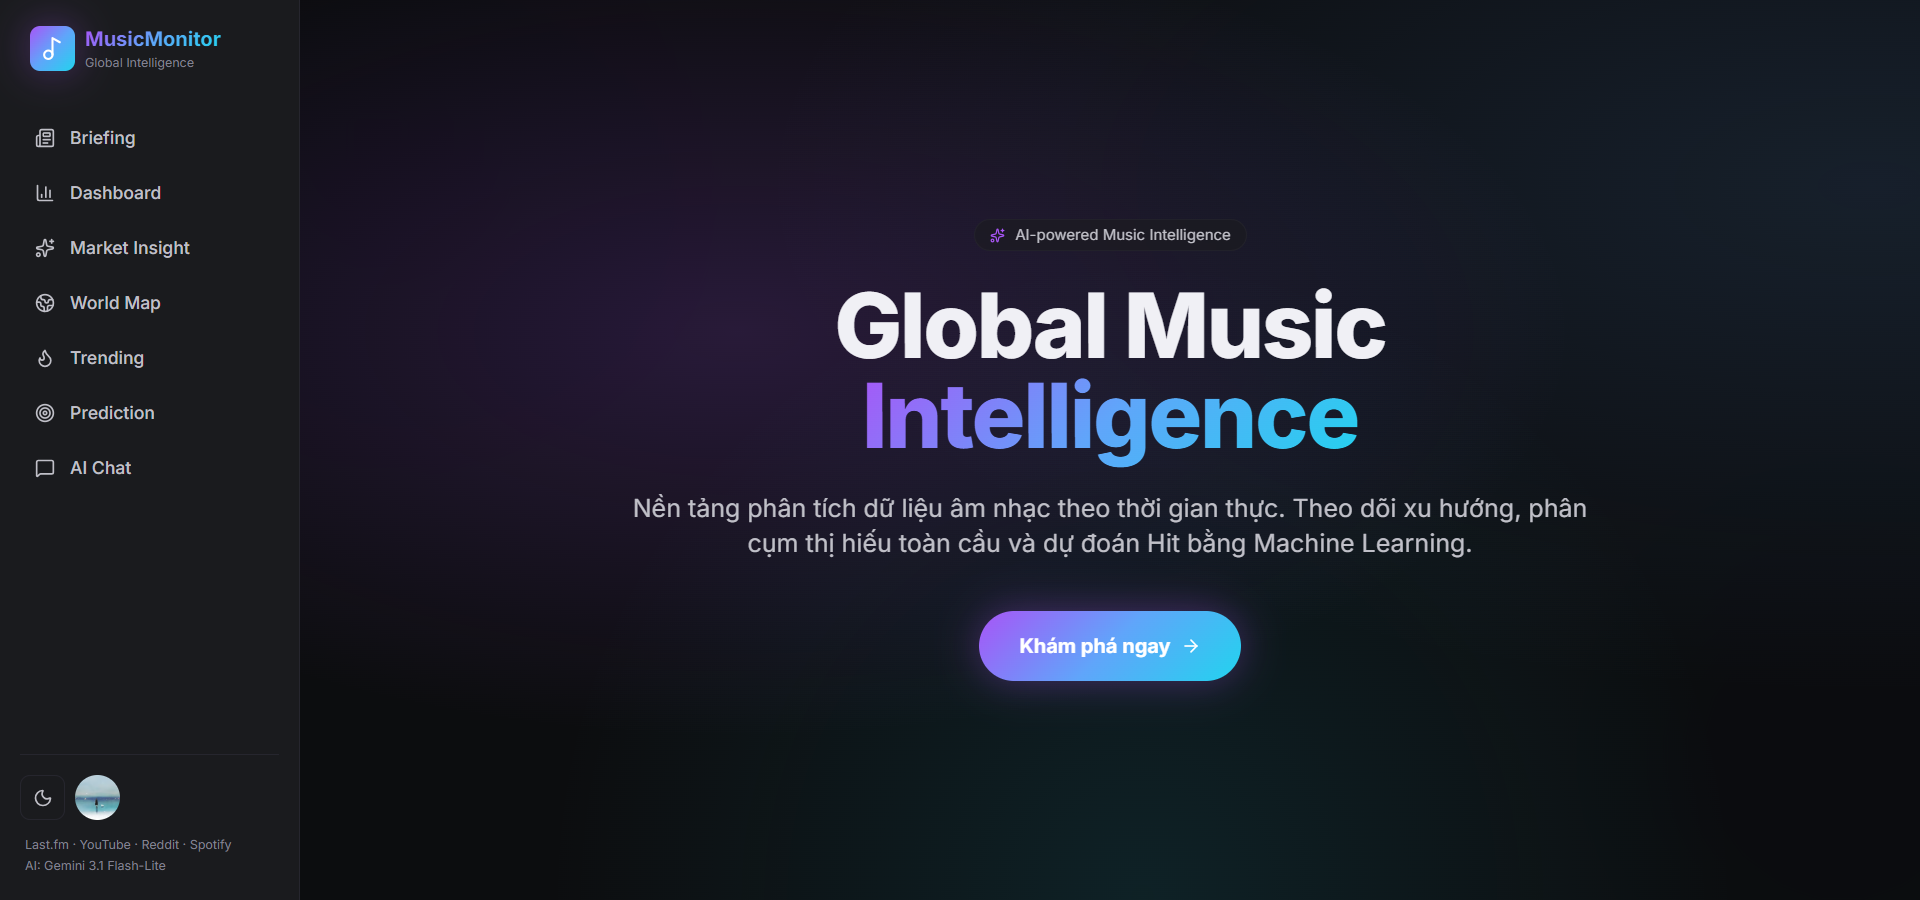
\includegraphics[width=\textwidth]{figures/landing-page.png}
    \caption{Giao diện Landing Page: Điểm chạm đầu tiên của người dùng với hệ thống Music Monitor}
    \label{fig:landing_page}
\end{figure}

\section{Dashboard - Giám sát Tổng quan}

Dashboard là màn hình trung tâm, cung cấp cái nhìn tổng thể về âm nhạc toàn cầu. Các thành phần chính:

\begin{itemize}
    \item \textbf{KPI Cards:} Số liệu nhanh (total charts, top track, viral score cao nhất, ...) được tính theo thời gian thực từ dữ liệu Firestore.
    \item \textbf{Global Top 50 Table:} Bảng xếp hạng hiển thị kèm điểm \textbf{MIS} (Music Intelligence Score), được tính như sau:
    \begin{itemize}
        \item \textbf{Dữ liệu đầu vào:} Tổng hợp từ \texttt{playcount} (tổng lượt nghe tích lũy) và \texttt{listeners} (lượng người nghe độc lập) của Last.fm.
        \item \textbf{Trọng số (Weight):} Vì playcount thường lớn gấp nhiều lần listeners, nó nghiễm nhiên trở thành trọng số chính khi cộng gộp cả hai.
        \item \textbf{Ý nghĩa:} Điểm số này giúp dễ dàng phân biệt các bài hát được nghe lại nhiều (playcount cao, listeners thấp) với các bài phổ biến nhưng ít nghe lại (listeners cao, playcount thấp).
    \end{itemize}
    \item \textbf{Live Anomaly Alert:} Phát hiện spike tự động bằng Z-score - công thức~\eqref{eq:zscore} - khi $Z > 2.5$.
    \item \textbf{Bộ lọc thời gian:} Today / This Week / This Month. Vì database mới khởi tạo, dữ liệu lịch sử thực chưa đủ cho filter tuần/tháng. Nhóm áp dụng mock shuffle \& scale playcount để demo UI - sau 3 tháng thu thập đủ, chỉ cần query Firestore theo timestamp.
    \item \textbf{Daily AI Briefing:} Tích hợp trực tiếp vào dashboard (xem mục 4.2).
\end{itemize}

\begin{figure}[H]
    \centering
    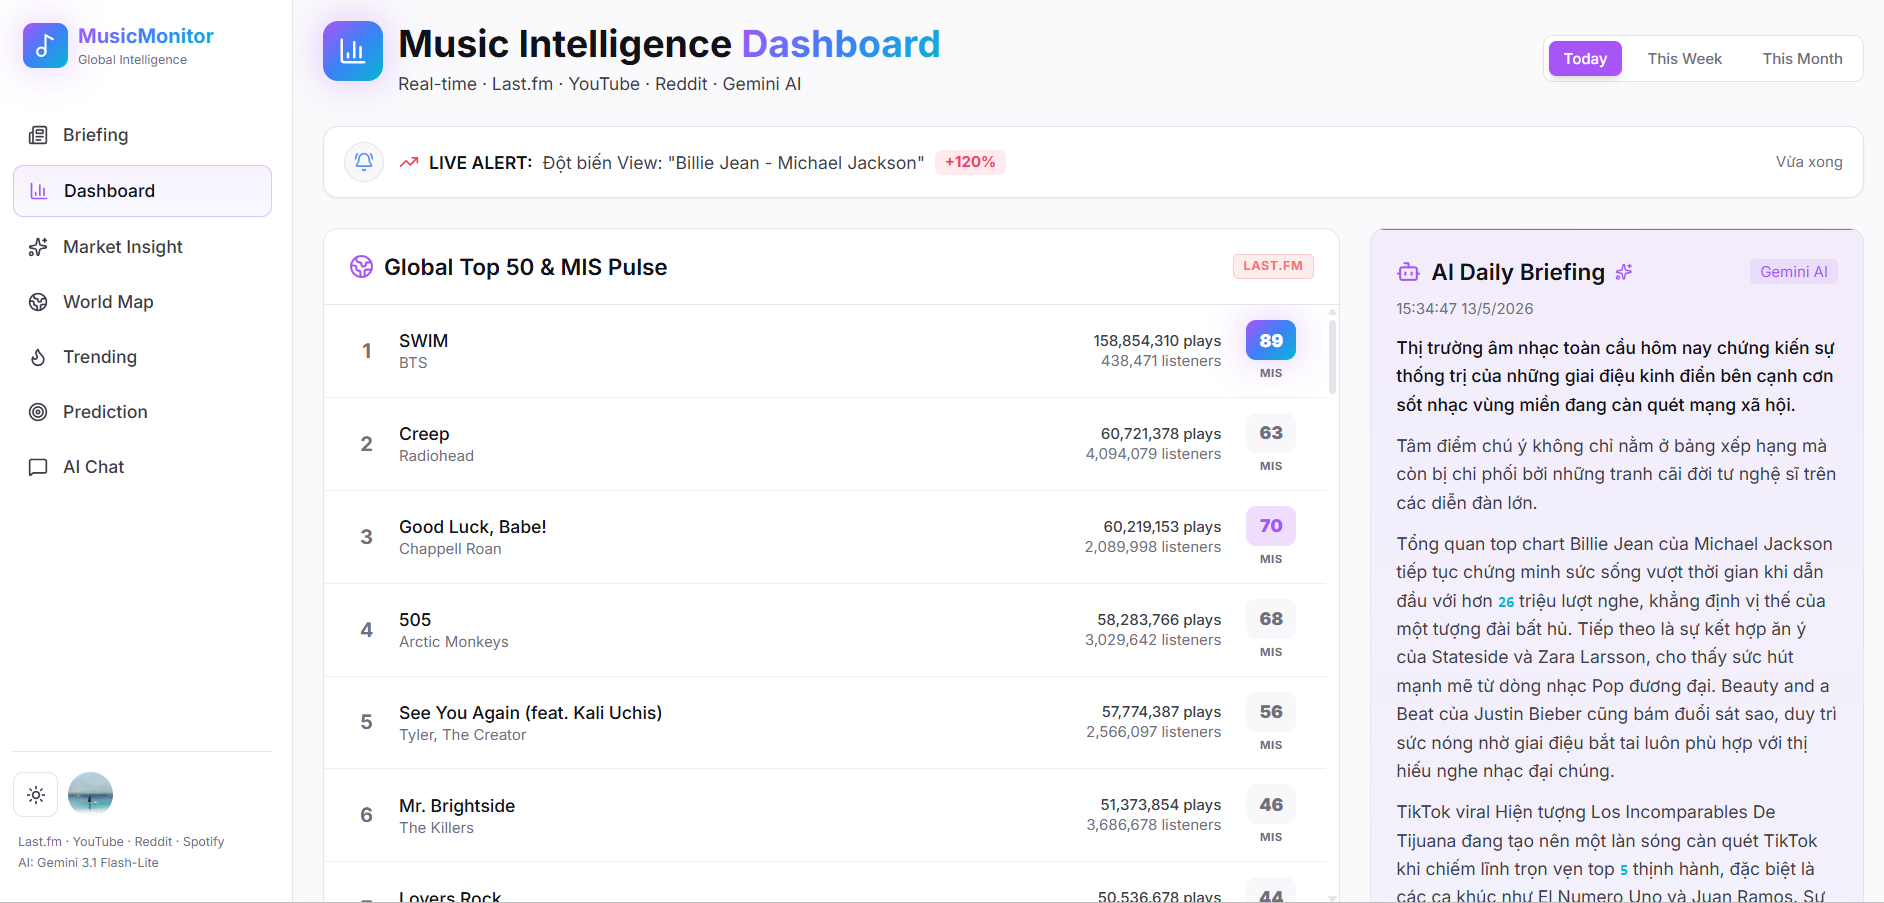
\includegraphics[width=\textwidth]{figures/dashboard.png}
    \caption{Dashboard chính: KPI Cards, Top 50 Chart, Anomaly Alert và Daily Briefing cạnh nhau}
    \label{fig:dashboard}
\end{figure}

\section{Daily Briefing \& Phân tích Cảm xúc}

\subsection{Pipeline Daily Briefing}

Daily Briefing tổng hợp bức tranh âm nhạc ngày hôm nay bằng cách kết hợp 3 nguồn dữ liệu qua Gemini AI:

\begin{enumerate}
    \item \textbf{Last.fm Top Charts:} Top 5 bài hát toàn cầu (tên, nghệ sĩ, playcount).
    \item \textbf{Reddit Sentiment (VADER NLP):} Phân tích cảm xúc cộng đồng từ hot posts trên r/Music, r/kpop, r/hiphopheads.
    \item \textbf{Deezer TikTok Viral:} Bài đang nổi TikTok với viral score.
\end{enumerate}

Ba nguồn được đóng gói thành JSON và gửi lên \textbf{Gemini 3.1 Flash-Lite} với prompt yêu cầu viết briefing 3 phần: Top Charts, Đang Viral, Dự báo. Kết quả được cache theo ngày (key \texttt{daily\_briefing\_legacy}) để không gọi Gemini nhiều lần.

\subsection{VADER Sentiment Analysis}

\textbf{VADER (Valence Aware Dictionary and sEntiment Reasoner)} là thư viện NLP phân tích cảm xúc văn bản. Hệ thống sử dụng VADER thay vì các mô hình deep learning (BERT, RoBERTa) vì ba đặc điểm phù hợp với bài toán:
\begin{itemize}
    \item VADER được thiết kế đặc biệt cho \textbf{social media text} (viết tắt, emoji, capslock, slang) - phù hợp với Reddit posts.
    \item Chạy trực tiếp không cần GPU, tốc độ nhanh cho real-time analysis.
    \item Cho ra compound score $\in [-1, 1]$ và phân loại Positive/Neutral/Negative.
\end{itemize}

Sơ đồ thuật toán phân tích cảm xúc (Sentiment Analysis) sử dụng VADER được thể hiện ở Hình~\ref{fig:vader_flow}.

\begin{figure}[H]
    \centering
    \resizebox{0.85\textwidth}{!}{
    \begin{tikzpicture}[
        node distance = 0.6cm and 1.2cm,
        box/.style = {draw, rectangle, rounded corners=5pt, minimum width=3.2cm, minimum height=1.0cm, align=center, font=\small\bfseries, line width=1pt},
        decision/.style = {draw, diamond, aspect=2.2, minimum width=3.2cm, minimum height=1.0cm, align=center, font=\small\bfseries, line width=1pt, fill=maccent!10, draw=maccent},
        process/.style = {box, fill=borderblue!6, draw=borderblue},
        input/.style = {box, fill=mgood!10, draw=mgood},
        loopbox/.style = {draw=black!40, dashed, rounded corners=8pt, line width=0.8pt, fill=black!2},
        arrow/.style = {draw=black!70, -{Stealth[scale=1.1]}, line width=1.1pt}
    ]

        % Input
        \node (input) [input] {Danh sách Reddit Posts\\(\texttt{posts})};
        
        % Loop Condition
        \node (checkPost) [decision, below=0.8cm of input] {Còn \texttt{post} nào\\chưa duyệt?};
        
        % Process Post
        \node (getScore) [process, below=0.8cm of checkPost] {Tính VADER Score\\từ \texttt{post["title"]}};
        \node (getCompound) [process, below=0.6cm of getScore] {Lấy \& Lưu điểm \texttt{compound}\\vào danh sách \texttt{scores}};
        
        % Decision
        \node (condPos) [decision, below=0.6cm of getCompound] {compound\\$> 0.05$?};
        \node (condNeg) [decision, below=0.6cm of condPos] {compound\\$< -0.05$?};
        
        % Actions
        \node (incPos) [process, right=of condPos] {\texttt{positive += 1}};
        \node (incNeg) [process, right=of condNeg] {\texttt{negative += 1}};
        
        % Loop End
        \node (loopEnd) [process, below=0.6cm of condNeg] {Chuyển sang bài tiếp theo};
        
        % Final calculation
        \node (calcFinal) [process, below=1.2cm of loopEnd] {Tính Tỷ lệ \% \& Trung bình:\\\texttt{positive\_pct}, \texttt{negative\_pct}};
        
        % Output
        \node (output) [input, below=0.6cm of calcFinal] {JSON Kết quả Sentiment\\(Truyền vào Prompt cho Gemini)};

        % Arrows Main Loop
        \draw [arrow] (input) -- (checkPost);
        \draw [arrow] (checkPost) -- node[anchor=east, font=\footnotesize\bfseries] {Đúng} (getScore);
        \draw [arrow] (getScore) -- (getCompound);
        \draw [arrow] (getCompound) -- (condPos);
        
        \draw [arrow] (condPos) -- node[anchor=east, font=\footnotesize\bfseries] {Sai} (condNeg);
        \draw [arrow] (condPos) -- node[anchor=south, font=\footnotesize\bfseries] {Đúng} (incPos);
        
        \draw [arrow] (condNeg) -- node[anchor=east, font=\footnotesize\bfseries] {Sai} (loopEnd);
        \draw [arrow] (condNeg) -- node[anchor=south, font=\footnotesize\bfseries] {Đúng} (incNeg);
        
        % Join actions to loopEnd
        \draw [arrow] (incPos.east) -- ++(0.5,0) |- (loopEnd.east);
        \draw [arrow] (incNeg.east) -- ++(0.5,0) |- (loopEnd.east);
        
        % Loop back
        \draw [arrow, dashed, -{Stealth[scale=1.1]}, line width=1.1pt] (loopEnd.west) -- ++(-1.5,0) |- (checkPost.west);
        
        % End Loop
        \coordinate (c2) at ($(incPos.east) + (1.2cm,0)$);
        \draw [arrow] (checkPost.east) -- node[anchor=south, font=\footnotesize\bfseries] {Sai (Hết)} (checkPost.east -| c2) |- (calcFinal.east);
        \draw [arrow] (calcFinal) -- (output);
        
        % Container for Loop
        \begin{scope}[on background layer]
            \node[loopbox, fit=(checkPost) (getScore) (getCompound) (condPos) (condNeg) (incPos) (incNeg) (loopEnd), label={[font=\sffamily\bfseries\color{borderblue}]above:Khối vòng lặp qua từng bài đăng (For loop)}] (loopBox) {};
        \end{scope}

    \end{tikzpicture}
    }
    \caption{Lưu đồ thuật toán Phân tích cảm xúc VADER cho Reddit Posts}
    \label{fig:vader_flow}
\end{figure}

\begin{figure}[H]
    \centering
    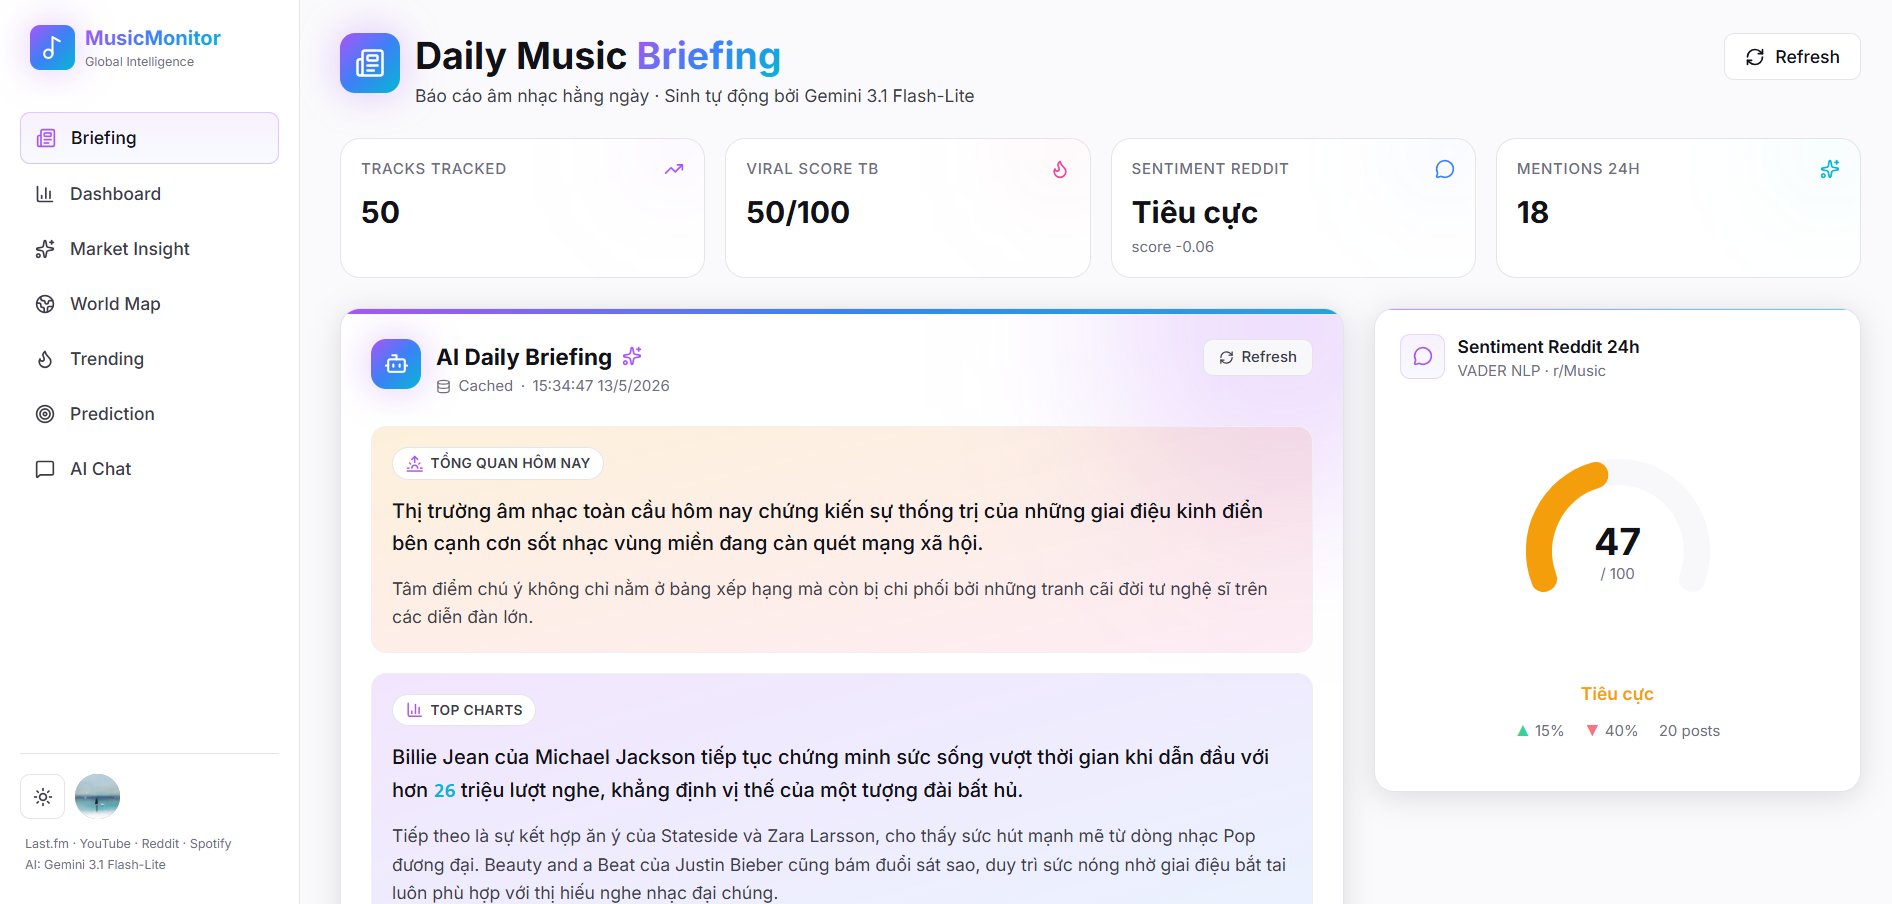
\includegraphics[width=\textwidth]{figures/daily-briefing.png}
    \caption{Daily Briefing tự động: VADER phân tích Reddit - JSON - Gemini AI viết bản tin}
    \label{fig:briefing}
\end{figure}

\section{Trending - Phát hiện Viral}

\subsection{Viral Score tổng hợp}

Hệ thống tính \textbf{Viral Score (0-100)} cho mỗi bài hát theo công thức có trọng số:

\begin{equation}
\text{Viral Score} = \min\!\left(\frac{G_{YT}}{500} \times 50, 50\right) + \min\!\left(\frac{M_{Reddit}}{100} \times 30, 30\right) + \min\!\left(\frac{C_{YT}}{50000} \times 20, 20\right)
\label{eq:viral_score}
\end{equation}

Trong đó:
\begin{itemize}
    \item $G_{YT}$: Tốc độ tăng trưởng view YouTube 24h (\%)
    \item $M_{Reddit}$: Số lần đề cập trên Reddit trong 24h
    \item $C_{YT}$: Tổng số comments YouTube MV
\end{itemize}

Giải thích các thành phần trọng số của công thức:
\begin{itemize}[leftmargin=*]
    \item \textbf{YouTube Views (50\%):} Phản ánh tốc độ viral nhanh và cung cấp số liệu tăng trưởng real-time chính xác nhất.
    \item \textbf{Reddit Mentions (30\%):} Đo lường mức độ thảo luận cộng đồng; đây thường là nơi bắt nguồn xu hướng sớm hơn cả các trang tin chính thống.
    \item \textbf{YouTube Comments (20\%):} Đo lường độ gắn kết chủ động (active engagement), tách biệt với lượt xem thụ động.
    \item \textbf{Mẫu số chuẩn hoá:} Các giá trị bão hoà ($500\%$, $100$ mentions, $50{,}000$ comments) được đúc kết từ thực tế: khi vượt qua các mốc này, bài hát đã đạt ngưỡng siêu viral.
\end{itemize}

\subsection{Z-score Spike Detection}

Để phát hiện spike bất thường trong lịch sử views YouTube, hệ thống dùng \textbf{Z-score}:

\begin{equation}
Z = \frac{x - \mu}{\sigma}
\label{eq:zscore}
\end{equation}

Cách hoạt động của thuật toán Z-score:
\begin{itemize}[leftmargin=*]
    \item \textbf{Cơ chế:} Đo lường sự lệch chuẩn của tốc độ tăng trưởng hiện tại ($x$) so với lịch sử tăng trưởng quá khứ ($\mu$, $\sigma$).
    \item \textbf{Ngưỡng bất thường ($Z > 2.5$):} Trong phân phối chuẩn, giá trị vượt 2.5 độ lệch chuẩn chỉ có 0.6\% xác suất xảy ra, tương đương một đợt tăng trưởng cực kỳ đột biến.
    \item \textbf{Xử lý thiếu dữ liệu:} Nếu chưa thu thập đủ 5 điểm lịch sử từ Firestore, hệ thống tự động sinh dữ liệu mô phỏng [55\%, 72\%, 88\%, 100\%] dựa trên lượt view hiện tại để Z-score vẫn hoạt động ổn định.
\end{itemize}

\subsection{Isolation Forest cho Anomaly Detection}

Nếu Z-score chỉ phân tích trên 1 chiều (views), thuật toán \textbf{Isolation Forest} giúp phát hiện bất thường đa chiều (tăng trưởng YouTube, Reddit mentions, comments, sentiment):
\begin{itemize}[leftmargin=*]
    \item \textbf{Phương pháp học (Unsupervised):} Hoạt động theo nguyên lý ``các điểm bất thường dễ bị phân lập'', rất phù hợp với dữ liệu không có nhãn sẵn.
    \item \textbf{Cấu hình (contamination=0.1):} Thiết lập tỷ lệ 10\% bài hát được kỳ vọng là bất thường (tương ứng với số lượng bài thật sự trending trong một bảng xếp hạng 50 bài).
    \item \textbf{Trực quan hoá:} Các bài bị đánh dấu $-1$ (anomaly) sẽ lập tức kích hoạt nhãn báo động ``Trending Anomaly'' trên Dashboard.
\end{itemize}

\subsection{Gemini Trend Explanation}

Sau khi phát hiện bài viral, hệ thống gọi Gemini để giải thích \textit{tại sao} bài đó viral. Prompt inject các chỉ số (growth \%, sentiment score, top Reddit post, genre) và yêu cầu giải thích 2-3 câu tiếng Việt. Kết quả cache theo key \texttt{trend:\{track\}:\{artist\}} (1 lần/ngày).

\begin{figure}[H]
    \centering
    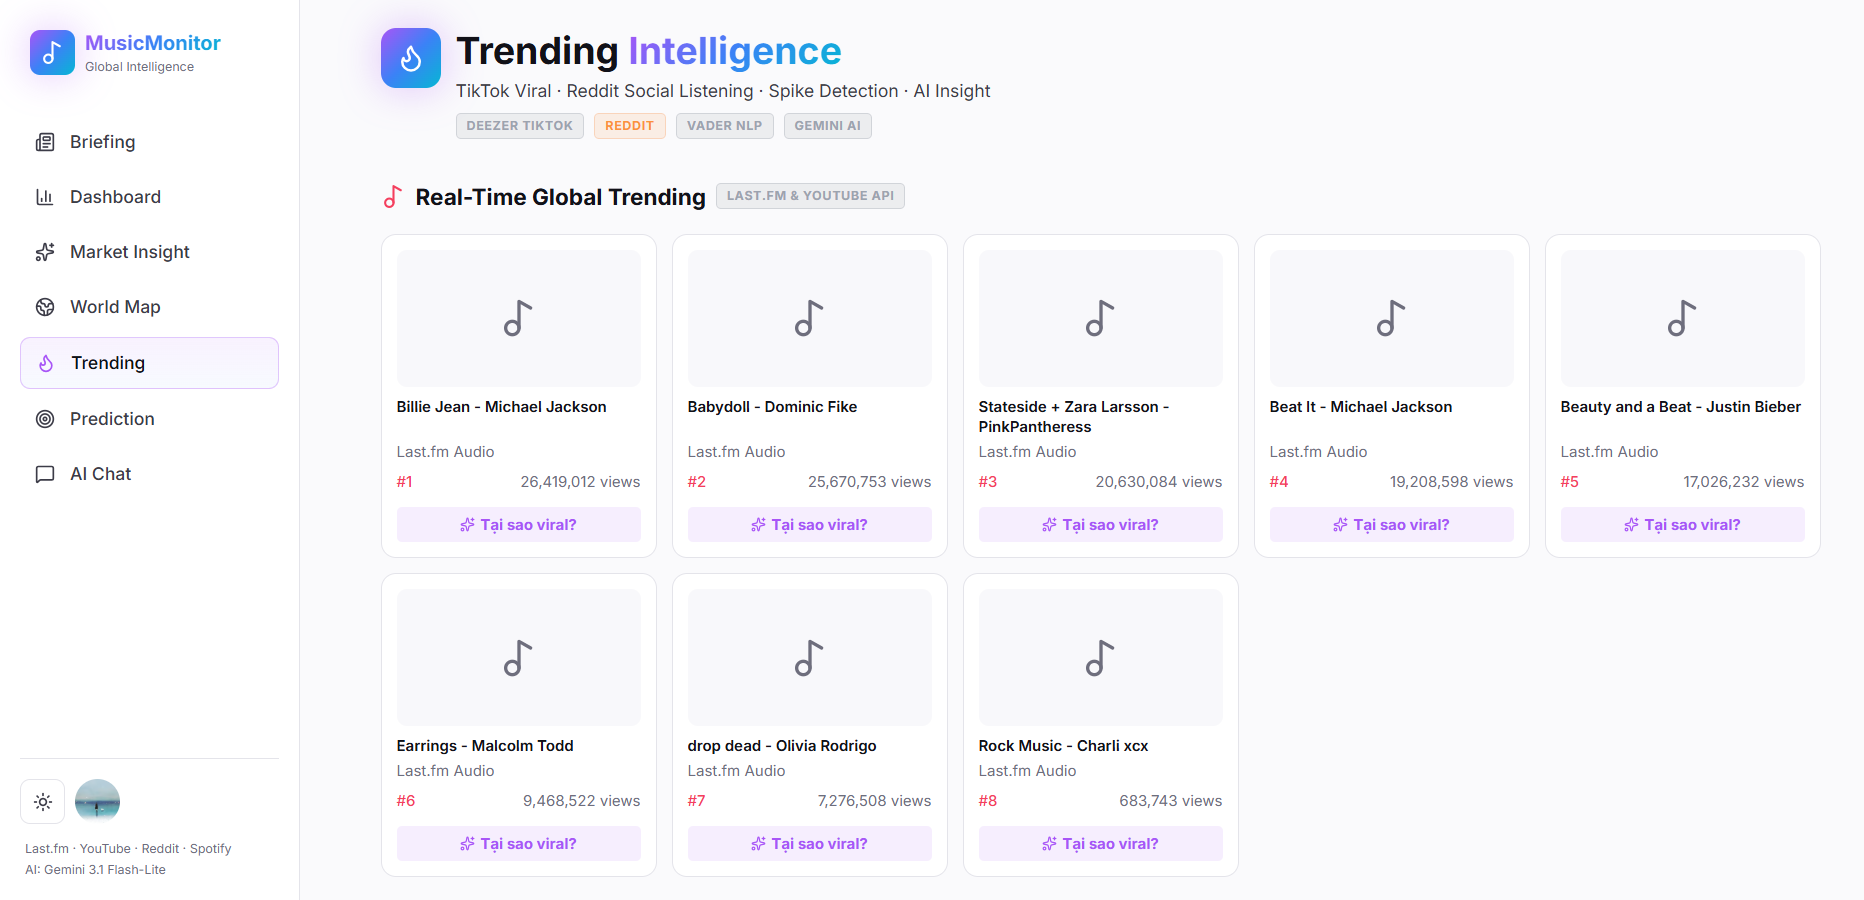
\includegraphics[width=\textwidth]{figures/visualize-trending.png}
    \caption{Trending page: Viral Score, Spike Detection, và AI Explanation cho từng bài hát}
    \label{fig:trending}
\end{figure}

\section{World Map - Phân cụm K-Means}

World Map trực quan hoá gu âm nhạc của 89 quốc gia bằng bản đồ tương tác. Mỗi quốc gia được tô màu theo cụm K-Means và khi click hiển thị AI Cultural Insight từ Gemini.

\begin{figure}[H]
    \centering
    
\includegraphics[width=\textwidth]{figures/global-map.png}
    \caption{World Music Map: 89 quốc gia phân cụm theo gu âm nhạc (K-Means, k=6)}
    \label{fig:worldmap}
\end{figure}

\textbf{Đặc điểm thú vị:} Kết quả clustering cho thấy Đông Nam Á có xu hướng cùng cụm với Latin America (cả hai đều ưa chuộng Pop/Dance/Latin), trong khi Đông Bắc Á (KR, JP, TW) tạo thành cụm K-Pop/J-Pop riêng biệt. Châu Phi (NG, GH, SN) tập trung vào cụm Afrobeats.

\section{Market Insight \& Phân tích Phân phối}

\subsection{Phân phối dữ liệu âm nhạc}

Dữ liệu âm nhạc có đặc tính \textbf{Pareto distribution} (quy luật 80/20): top 1\% bài hát chiếm áp đảo lượng nghe. Điều này được quan sát qua:
\begin{itemize}
    \item Histogram playcount Last.fm: đuôi nặng phải (heavy right tail), skewness rất lớn.
    \item Scatter plot YouTube Views vs Reddit Upvotes: cluster dày ở góc dưới trái, vài điểm ngoại lệ ở góc trên phải.
\end{itemize}

\textbf{Ý nghĩa kỹ thuật:} Khi đưa dữ liệu vào mô hình ML (đặc biệt XGBoost), cần áp dụng \textbf{Log-Transform} để cân bằng phân phối. Trong pipeline hit prediction, các đặc trưng \texttt{youtube\_views}, \texttt{lastfm\_playcount}, \texttt{artist\_playcount} đều được scale trước khi đưa vào XGBoost.

\begin{figure}[H]
    \centering
    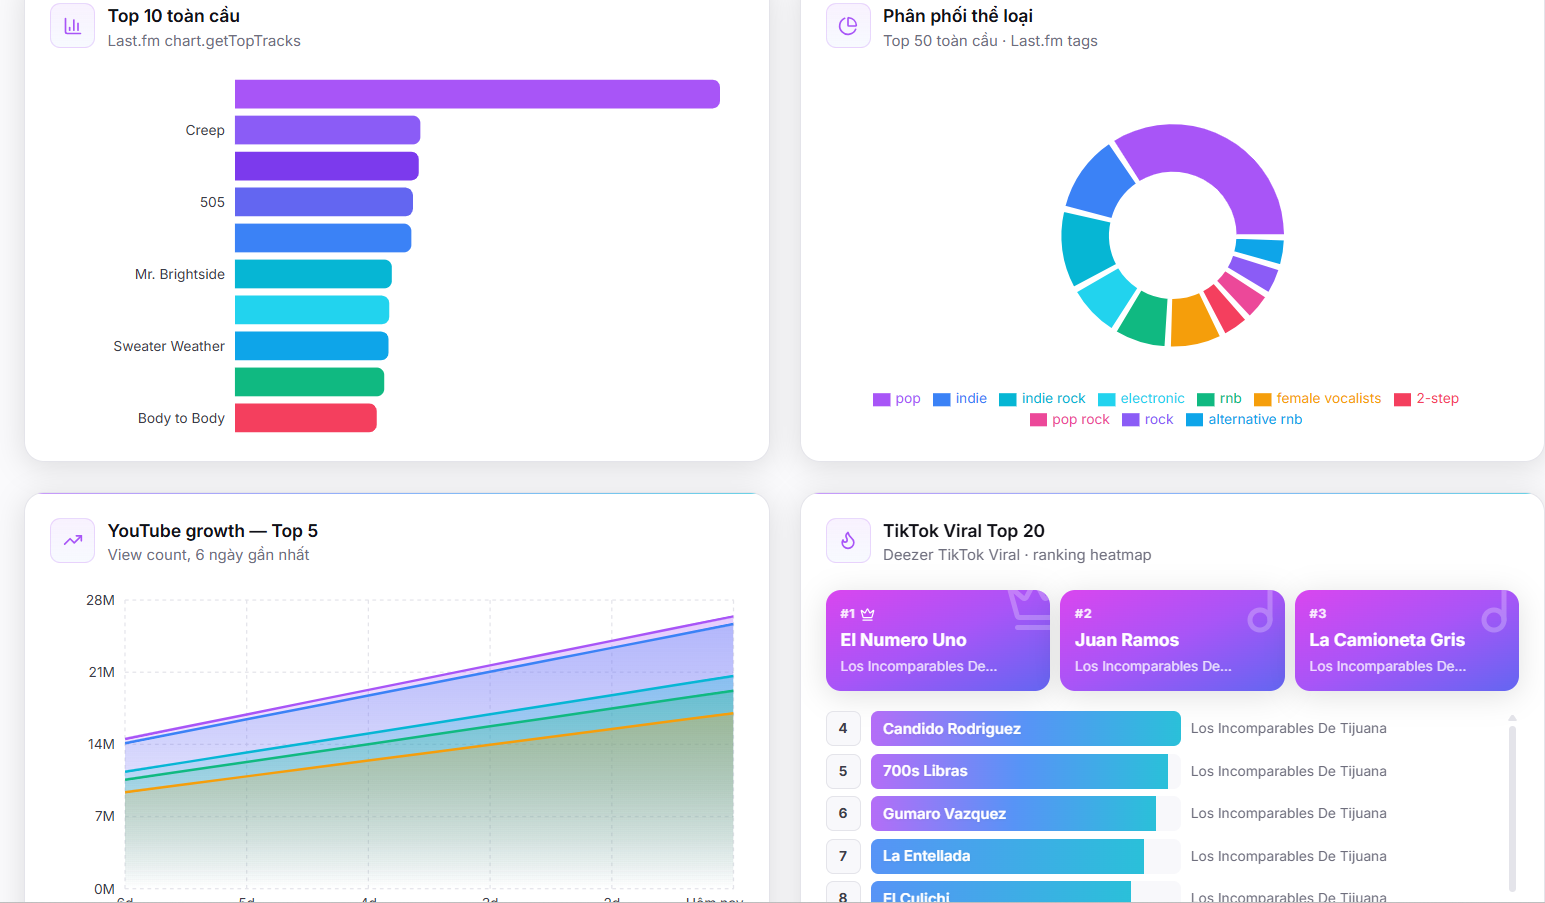
\includegraphics[width=\textwidth]{figures/phan-phoi-dl.png}
    \caption{Phân phối dữ liệu âm nhạc: Pareto distribution, cross-platform correlation, và sentiment bar}
    \label{fig:distribution}
\end{figure}

\begin{figure}[H]
    \centering
    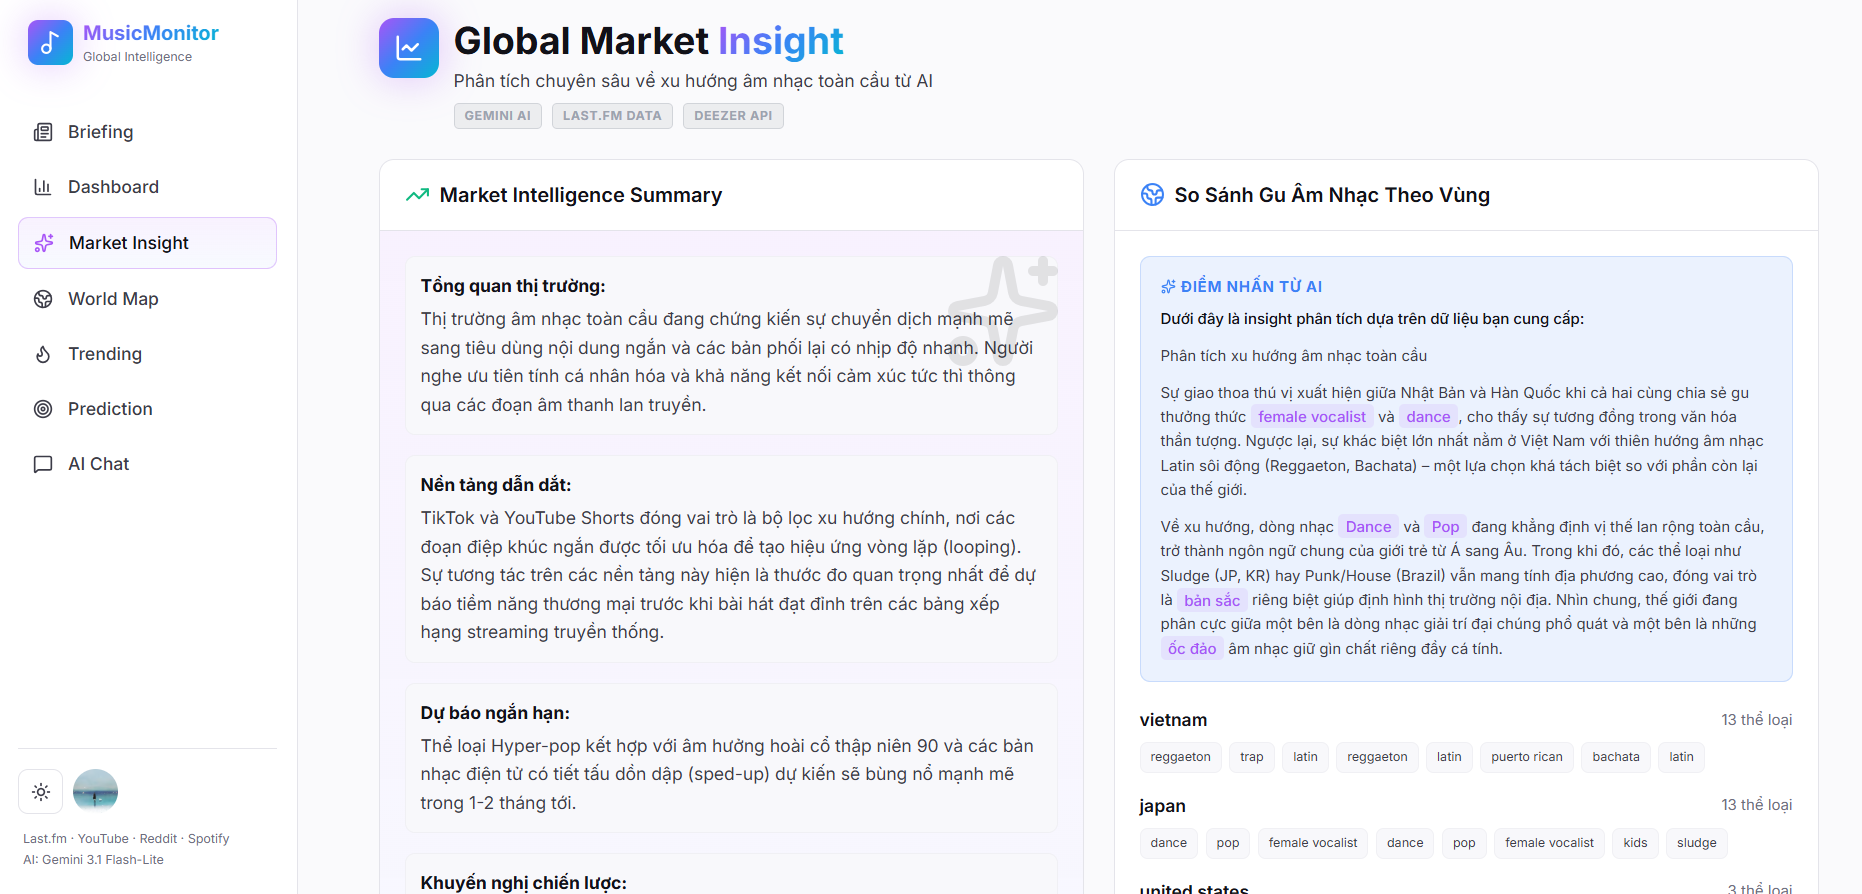
\includegraphics[width=\textwidth]{figures/market-insight.png}
    \caption{Market Insight: tổng hợp đa nguồn, hit score, radar đặc trưng, và buzz analytics}
    \label{fig:market_insight}
\end{figure}

\section{Social Listening}

Social Listening theo dõi cộng đồng Reddit (r/Music, r/kpop, r/hiphopheads, ...) để nắm bắt phản ứng người nghe theo thời gian thực.

\begin{itemize}
    \item \textbf{Multi-subreddit monitoring:} Theo dõi đồng thời nhiều subreddit, lọc bài hot trong 24h.
    \item \textbf{VADER NLP:} Phân loại cảm xúc mỗi post (Positive/Neutral/Negative).
    \item \textbf{Mentions 24h counter:} Đếm số lần đề cập một nghệ sĩ/bài hát trong 24h để phát hiện sớm khủng hoảng truyền thông.
    \item \textbf{Gemini AI Insight:} Phân tích chủ đề chính, mức độ quan tâm, góc nhìn cộng đồng từ tiêu đề bài post.
\end{itemize}

\begin{figure}[H]
    \centering
    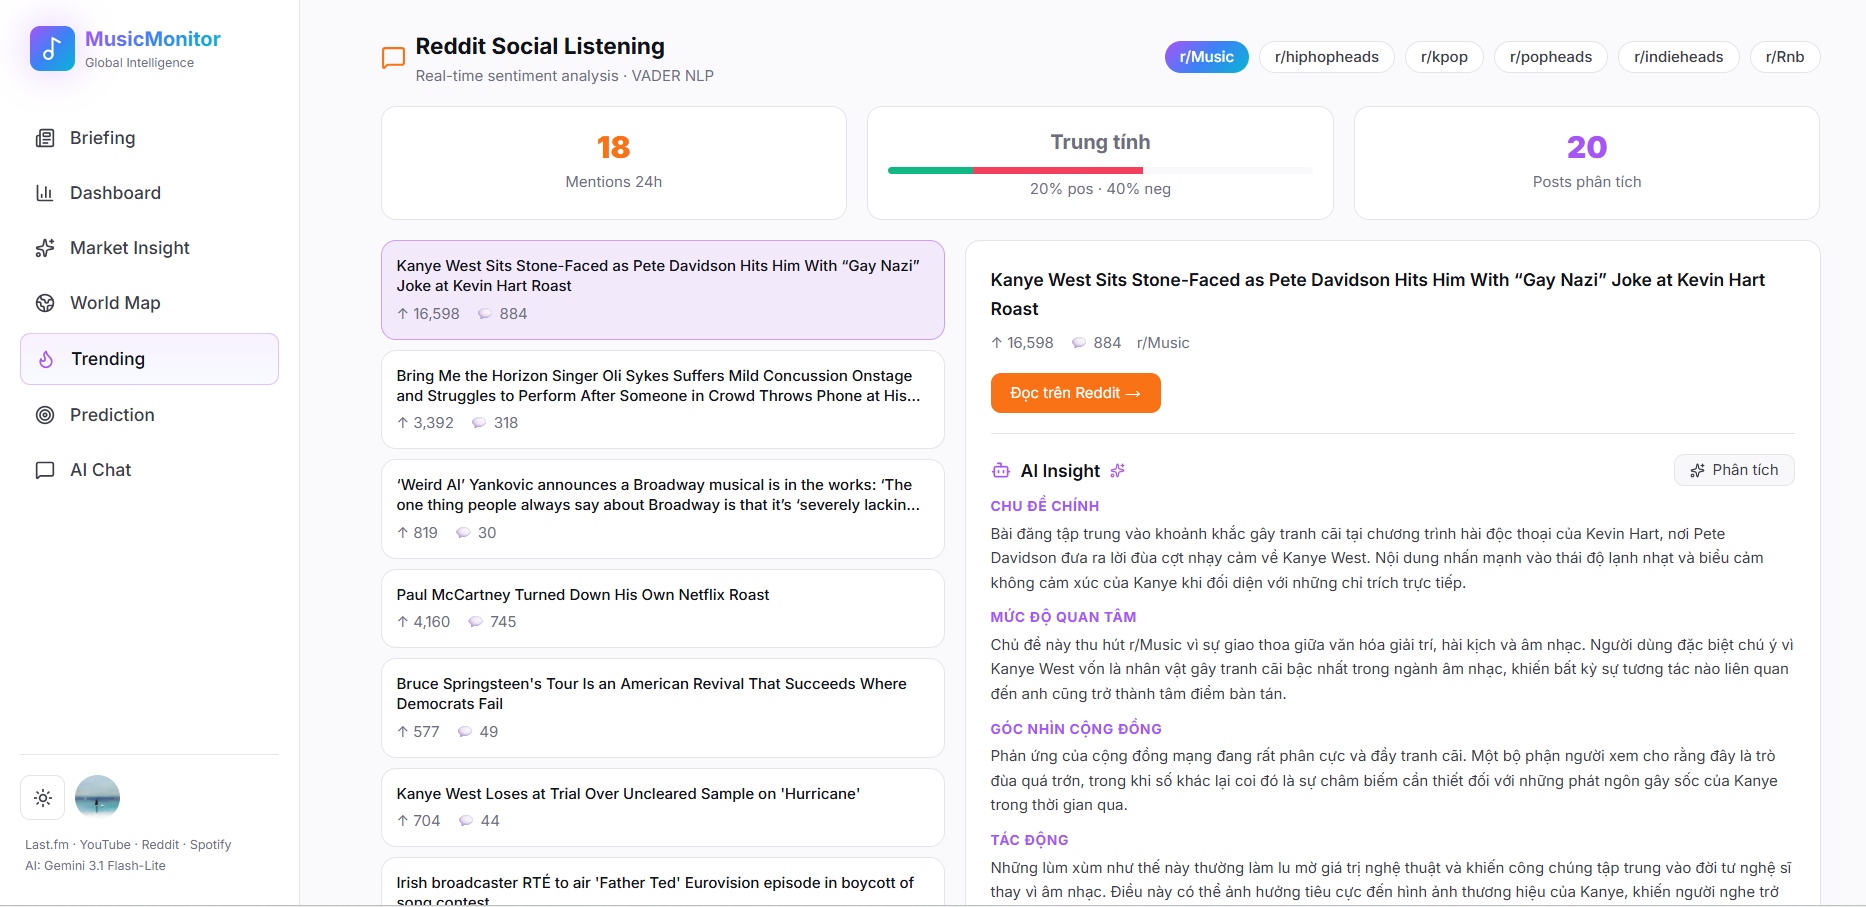
\includegraphics[width=\textwidth]{figures/social-listening.png}
    \caption{Social Listening: Reddit monitoring, VADER sentiment, và AI analysis}
    \label{fig:social_listening}
\end{figure}

% ============================================================
% CHƯƠNG 5 — DỰ ĐOÁN HIT VÀ AI AGENT
% ============================================================
\chapter{DỰ ĐOÁN HIT VÀ AI AGENT}

\section{Mô hình Dự đoán Hit (XGBoost)}

\subsection{Thiết kế đặc trưng (Feature Engineering)}

Mô hình dự đoán bài hát có trở thành hit hay không trong 7 ngày tới. Vector đặc trưng gồm \textbf{11 chiều}:

\begin{table}[H]
\centering
\caption{Vector đặc trưng đầu vào mô hình XGBoost}
\label{tab:features}
\begin{tabular}{|l|l|l|}
\hline
\textbf{Đặc trưng} & \textbf{Nguồn} & \textbf{Ý nghĩa} \\
\hline
\texttt{youtube\_growth\_24h} & YouTube Data API & \% tăng view trong 24h \\
\texttt{youtube\_growth\_48h} & YouTube Data API & \% tăng view trong 48h \\
\texttt{youtube\_growth\_7d} & YouTube Data API & \% tăng view trong 7 ngày \\
\texttt{reddit\_mentions\_24h} & Reddit API & Số đề cập Reddit 24h \\
\texttt{youtube\_comments} & YouTube Data API & Tổng comments MV \\
\texttt{lastfm\_playcount} & Last.fm API & Tổng lượt nghe Last.fm \\
\texttt{lastfm\_listeners} & Last.fm API & Số người nghe Last.fm \\
\texttt{genre\_popularity} & Last.fm artist.getTopTags & Điểm popularity thể loại (0-1) \\
\texttt{artist\_playcount} & Last.fm API & Tổng lượt nghe nghệ sĩ \\
\texttt{month} & System & Tháng hiện tại (seasonality) \\
\texttt{is\_holiday\_season} & System & Flag mùa lễ tết (11, 12, 1) \\
\hline
\end{tabular}
\end{table}

Bên cạnh các chỉ số tương tác thông thường, hệ thống đặc biệt chú trọng vào 2 nhóm đặc trưng bổ sung để tăng độ nhạy (sensitivity) của mô hình:
\begin{itemize}[leftmargin=*]
    \item \textbf{Yếu tố thời vụ (Seasonality):} Dữ liệu âm nhạc chịu ảnh hưởng mạnh bởi thời gian. Tháng 11-12 (Black Friday, Giáng sinh) và tháng 1 (Tết Âm lịch) thường có độ biến động bảng xếp hạng cực cao do các đợt phát hành album ồ ạt. Các đặc trưng \texttt{month} và \texttt{is\_holiday\_season} giúp mô hình nhận diện được bối cảnh thời gian, tránh việc đánh đồng mức độ viral của một bài hát trong tháng 7 (mùa thấp điểm) với tháng 12 (mùa cao điểm).
    \item \textbf{Sức hút thể loại (Genre Popularity):} Một số dòng nhạc đại chúng (pop, hip-hop, k-pop) luôn có lợi thế thống trị bảng xếp hạng cao hơn dòng nhạc ngách (jazz, classical). Hệ thống chuẩn hoá \texttt{genre\_popularity} về đoạn $[0, 1]$ với công thức: \texttt{genre\_score = len([t for t in tags if t in high\_pop]) / 3} (cắt tại giới hạn 1.0). Thiết kế này giúp mô hình hiểu được lợi thế khởi điểm của một bài hip-hop so với bài classical kể cả khi cả hai có cùng các chỉ số lượt nghe ban đầu.
\end{itemize}

\begin{figure}[H]
    \centering
    \resizebox{0.95\textwidth}{!}{
    \begin{tikzpicture}[
        node distance = 0.8cm and 1.2cm,
        box/.style = {draw, rectangle, rounded corners=5pt, minimum width=2.5cm, minimum height=1.0cm, align=center, font=\small\bfseries, line width=1pt},
        source/.style = {box, fill=borderblue!10, draw=borderblue},
        process/.style = {box, fill=maccent!10, draw=maccent},
        output/.style = {box, fill=mgood!10, draw=mgood, minimum width=3.5cm},
        arrow/.style = {draw=black!70, -{Stealth[scale=1.1]}, line width=1.1pt}
    ]

        % Sources
        \node (yt) [source] {YouTube API};
        \node (reddit) [source, below=of yt] {Reddit API};
        \node (lastfm) [source, below=of reddit] {Last.fm API};
        \node (sys) [source, below=of lastfm] {System Clock};

        % Processes
        \node (p_yt) [process, right=of yt] {Tính \% Growth\\\& Đếm Comments};
        \node (p_reddit) [process, right=of reddit] {Đếm số Mentions\\trong 24h};
        \node (p_lastfm) [process, right=of lastfm] {Trích xuất Lượt nghe\\\& Phân tích Genre};
        \node (p_sys) [process, right=of sys] {Trích xuất Tháng\\\& Nhãn Holiday};

        % Concat
        \node (concat) [process, right=1.5cm of p_reddit, yshift=-0.8cm, minimum height=4cm, minimum width=1.5cm, fill=black!5, draw=black!50] {Hợp nhất\\(Concat)};

        % Vector
        \node (vector) [output, right=1.5cm of concat] {Vector 11 chiều\\$\mathbf{x} = [x_1, x_2, ..., x_{11}]$};

        % XGBoost
        \node (xgb) [output, right=1.5cm of vector, fill=mprimary!20, draw=mprimary] {XGBoost Classifier};

        % Arrows
        \draw [arrow] (yt) -- (p_yt);
        \draw [arrow] (reddit) -- (p_reddit);
        \draw [arrow] (lastfm) -- (p_lastfm);
        \draw [arrow] (sys) -- (p_sys);
        
        \draw [arrow] (p_yt.east) -- ++(0.5,0) |- (concat.west);
        \draw [arrow] (p_reddit.east) -- ++(0.5,0) |- (concat.west);
        \draw [arrow] (p_lastfm.east) -- ++(0.5,0) |- (concat.west);
        \draw [arrow] (p_sys.east) -- ++(0.5,0) |- (concat.west);

        \draw [arrow] (concat) -- (vector);
        \draw [arrow] (vector) -- (xgb);

    \end{tikzpicture}
    }
    \caption{Sơ đồ quy trình trích xuất và biến đổi đặc trưng (Feature Engineering Pipeline)}
    \label{fig:feature_pipeline}
\end{figure}

\subsection{Kiến trúc và huấn luyện XGBoost}

Mô hình XGBoost được huấn luyện trên \textbf{Kaggle} (notebook \texttt{music-monitor-eda-training.ipynb}):

Sơ đồ thiết lập cấu hình siêu tham số (Hyperparameters) cho mô hình XGBoost được thể hiện ở Hình~\ref{fig:xgboost_config}.

\begin{figure}[H]
    \centering
    \resizebox{0.9\textwidth}{!}{
    \begin{tikzpicture}[
        node distance = 1.5cm and 2.0cm,
        box/.style = {draw, rectangle, rounded corners=5pt, align=center, line width=1pt},
        mainnode/.style = {box, fill=mprimary!10, draw=mprimary, minimum width=4.5cm, minimum height=1.5cm, font=\large\bfseries\sffamily},
        parambox/.style = {box, fill=borderblue!6, draw=borderblue, minimum width=4.0cm, minimum height=1.0cm, font=\small\ttfamily},
        arrow/.style = {draw=black!60, -{Stealth[scale=1.1]}, line width=1.2pt, dashed}
    ]

        % Central Node
        \node (xgboost) [mainnode] {XGBClassifier};
        
        % Parameter Groups
        \node (trees) [parambox, above=1.5cm of xgboost, label={[font=\small\bfseries\sffamily\color{borderblue}]above:Kiểm soát Cấu trúc Cây (Tree Structure)}] {n\_estimators = 300\\max\_depth = 6};
        
        \node (learning) [parambox, left=1.8cm of xgboost, label={[font=\small\bfseries\sffamily\color{borderblue}]above:Quá trình Học (Learning)}] {learning\_rate = 0.05\\eval\_metric = "logloss"};
        
        \node (sampling) [parambox, right=1.8cm of xgboost, label={[font=\small\bfseries\sffamily\color{borderblue}]above:Lấy mẫu chống Overfit (Sampling)}] {subsample = 0.8\\colsample\_bytree = 0.8};
        
        \node (random) [parambox, below=1.5cm of xgboost, label={[font=\small\bfseries\sffamily\color{borderblue}]above:Khởi tạo (Reproducibility)}] {random\_state = 42};
        
        % Connections
        \draw [arrow] (trees) -- (xgboost);
        \draw [arrow] (learning) -- (xgboost);
        \draw [arrow] (sampling) -- (xgboost);
        \draw [arrow] (random) -- (xgboost);

    \end{tikzpicture}
    }
    \caption{Cấu hình siêu tham số (Hyperparameters) cho mô hình XGBoost Hit Prediction}
    \label{fig:xgboost_config}
\end{figure}


\textbf{Dữ liệu huấn luyện:} 5.000 mẫu synthetic (vì dữ liệu hit thực tế khó thu thập và rất imbalanced). Nhãn \texttt{is\_hit=1} khi đồng thời: \texttt{youtube\_growth\_24h > 100} AND \texttt{reddit\_mentions\_24h > 20} AND \texttt{lastfm\_listeners > 100.000}. Tỷ lệ hit: $\approx 0.2\%$ (rất imbalanced - nhưng XGBoost xử lý tốt với \texttt{eval\_metric=logloss}).

\textbf{Kết quả đánh giá trên tập test (20\%):}
\begin{itemize}
    \item ROC AUC: \textbf{1.0000} (do dữ liệu synthetic với decision boundary rõ ràng)
    \item Precision/Recall Normal: 1.00/1.00
    \item F1-score macro avg: 0.75 (bị ảnh hưởng bởi class imbalance của nhãn Hit)
\end{itemize}

\begin{figure}[H]
    \centering
    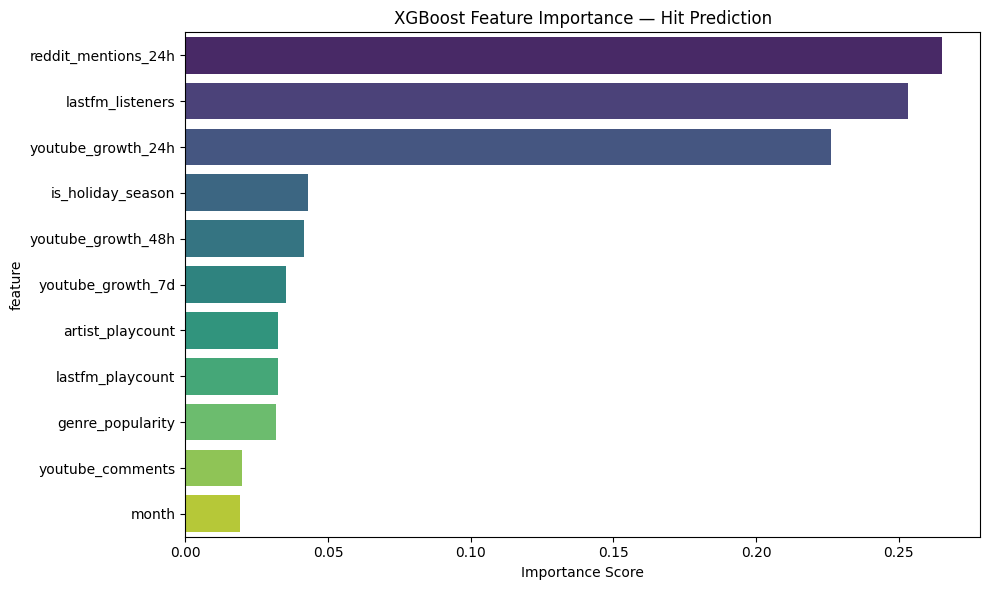
\includegraphics[width=0.8\textwidth]{figures/feature-importance.png}
    \caption{Feature Importance XGBoost: youtube\_growth\_24h và lastfm\_listeners là đặc trưng quan trọng nhất}
    \label{fig:feature_importance}
\end{figure}

\subsection{Xác suất dự đoán và công thức tính}

Hàm \texttt{predict\_hit\_\allowbreak{}probability()} trả về xác suất hit bằng \textbf{XGBoost's \allowbreak{}predict\_proba}:

\begin{equation}
P(\text{hit}) = \text{XGBoost.predict\_proba}(\mathbf{x})[0][1]
\label{eq:hit_prob}
\end{equation}

Xác suất này được tính bằng hàm sigmoid trên output của cây quyết định ensemble:
\begin{equation}
P(\text{hit}) = \frac{1}{1 + e^{-F(\mathbf{x})}}
\label{eq:sigmoid}
\end{equation}
trong đó $F(\mathbf{x}) = \sum_{k=1}^{K} f_k(\mathbf{x})$ là tổng output của K cây quyết định (K=300).

\textbf{Fallback Heuristic:} Khi model file (\texttt{hit\_predictor.joblib}) không tồn tại, hệ thống dùng heuristic:
\begin{equation}
P_{\text{heuristic}} = \min\!\left(\frac{G_{YT}}{1000} \times 0.6 + \frac{M_{Reddit}}{200} \times 0.4,\; 0.99\right)
\label{eq:heuristic}
\end{equation}

\textbf{Phân loại kết quả:}
\begin{itemize}
    \item $P > 0.6$: ``Potential Hit'' (cao)
    \item $0.3 < P \leq 0.6$: ``Watch'' (trung bình, cần theo dõi)
    \item $P \leq 0.3$: ``Normal'' (thấp)
\end{itemize}

\subsection{Quick Prediction Pipeline}

Khi người dùng nhập tên bài + nghệ sĩ, backend tự động:
\begin{enumerate}
    \item Tìm metadata từ \textbf{Deezer} (ảnh bìa, preview 30s, normalised track name).
    \item Tìm MV YouTube và lấy view stats + áp dụng decay factor.
    \item Đếm Reddit mentions 24h.
    \item Tính genre\_popularity từ Last.fm artist tags.
    \item Gọi \texttt{predict\_hit\_\allowbreak{}probability()} và trả kết quả kèm audio preview.
\end{enumerate}

\begin{figure}[H]
    \centering
    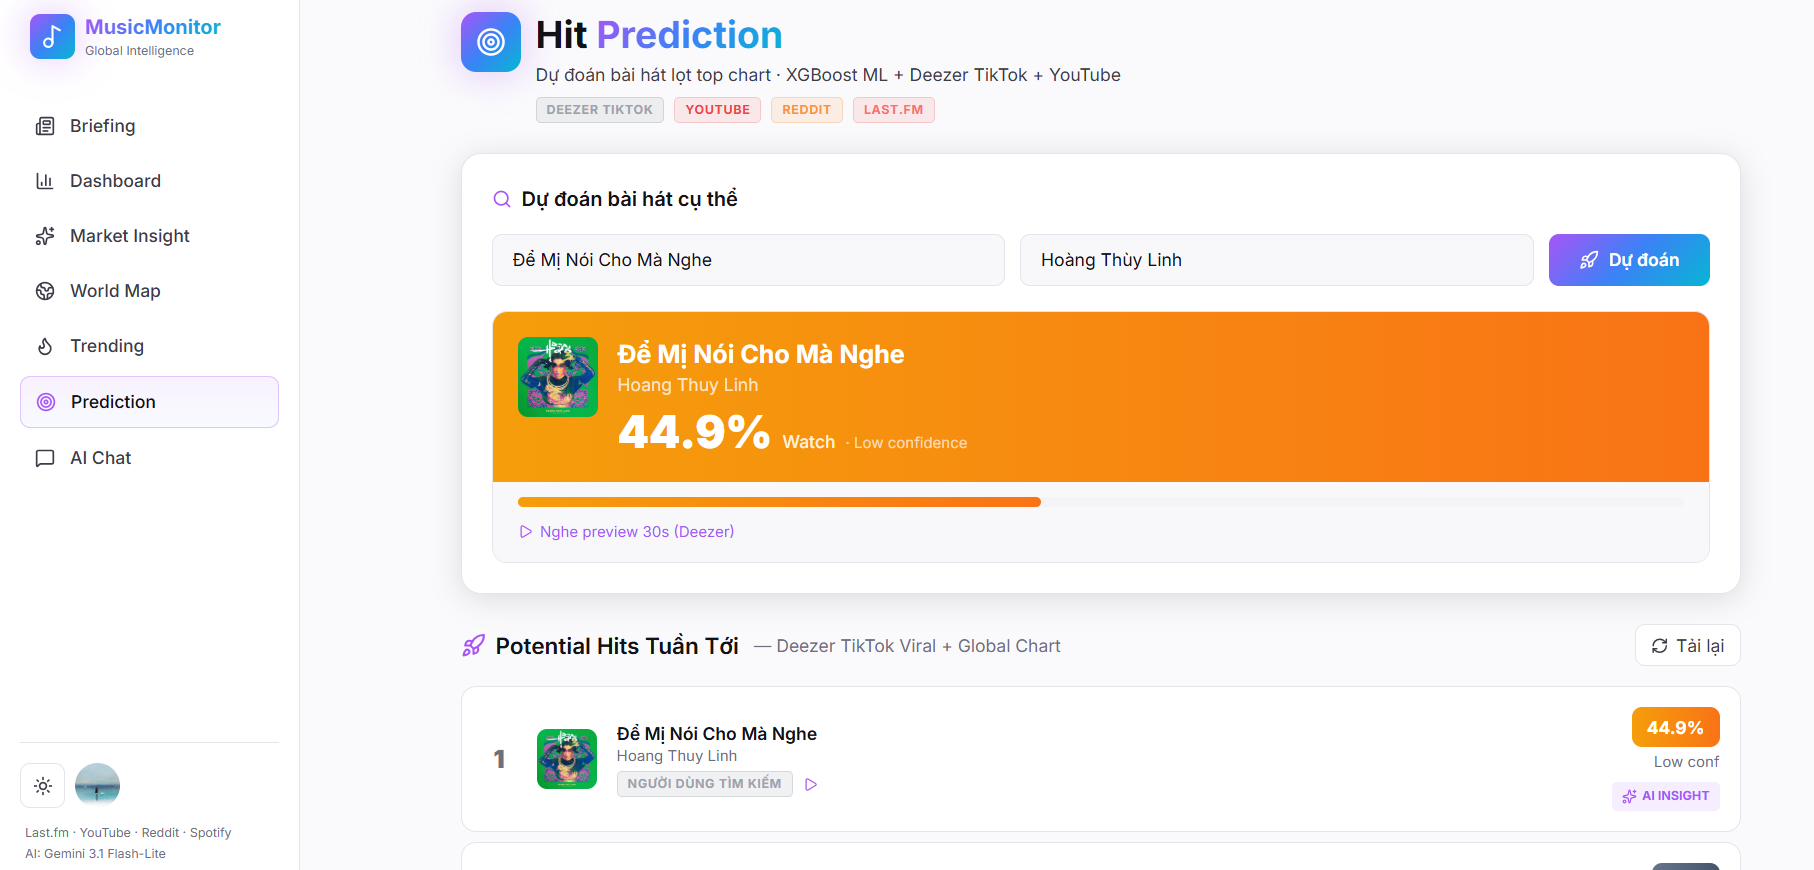
\includegraphics[width=\textwidth]{figures/hit-prediction.png}
    \caption{Hit Prediction UI: Nhập URL/tên bài, pipeline tự thu thập, XGBoost dự đoán kèm audio preview}
    \label{fig:hit_prediction}
\end{figure}

\section{Giải thích Dự đoán (Explainable AI)}

Một trong những thách thức lớn nhất của ML trong thực tế là ``hộp đen'': mô hình cho ra xác suất nhưng không giải thích \textit{tại sao}. Hệ thống giải quyết vấn đề này bằng pipeline \textbf{Explainable AI} 4 tầng, biến output số của XGBoost thành lời khuyên hành động cụ thể bằng ngôn ngữ tự nhiên.

Sơ đồ pipeline Explainable AI được trình bày ở Hình~\ref{fig:xai_pipeline}.

\begin{figure}[H]
    \centering
    \resizebox{\textwidth}{!}{
    \begin{tikzpicture}[
        node distance = 0.7cm and 1.2cm,
        box/.style = {draw, rectangle, rounded corners=5pt, minimum width=2.6cm, minimum height=1.0cm, align=center, font=\small\bfseries, line width=1pt},
        model/.style = {box, fill=mprimary!10, draw=mprimary},
        process/.style = {box, fill=borderblue!6, draw=borderblue},
        ai/.style = {box, fill=maccent!10, draw=maccent},
        result/.style = {box, fill=mgood!10, draw=mgood},
        arrow/.style = {draw=black!70, -{Stealth[scale=1.1]}, line width=1.1pt}
    ]

        % Row 1: XGBoost output
        \node (xgb) [model] {XGBoost Output\\$P(\text{hit}) = 44.9\%$};

        % Row 2: 3 parallel analysis branches
        \node (rank) [process, below=0.8cm of xgb] {Feature Rank\\(Contribution +/-)};
        \node (shap) [process, left=0.5cm of rank] {SHAP Weights\\(Feature Importance)};
        \node (radar) [process, right=0.5cm of rank] {Radar 5 trục\\(Hit Formula)};

        % Row 3: Gemini
        \node (gemini) [ai, below=1.0cm of rank] {Gemini AI\\Phiên dịch ngữ nghĩa};

        % Row 4: Outputs
        \node (risk) [result, below=0.8cm of gemini] {Risk Tier\\(High/Watch/Normal)};
        \node (narrative) [result, left=0.5cm of risk] {Narrative\\(Giải thích NLP)};
        \node (action) [result, right=0.5cm of risk] {Action Plan\\(Chiến lược)};

        % Arrows XGBoost -> Branches
        \coordinate (split1) at ($(xgb.south) + (0,-0.4)$);
        \draw [line width=1.1pt, draw=black!70] (xgb.south) -- (split1);
        \draw [arrow] (split1) -| (shap.north);
        \draw [arrow] (split1) -| (radar.north);
        \draw [arrow] (split1) -- (rank.north);

        % Arrows Branches -> Gemini
        \coordinate (merge1) at ($(gemini.north) + (0,0.5)$);
        \draw [line width=1.1pt, draw=black!70] (shap.south) |- (merge1);
        \draw [line width=1.1pt, draw=black!70] (radar.south) |- (merge1);
        \draw [line width=1.1pt, draw=black!70] (rank.south) -- (merge1);
        \draw [arrow] (merge1) -- (gemini.north);

        % Arrows Gemini -> Outputs
        \coordinate (split2) at ($(gemini.south) + (0,-0.4)$);
        \draw [line width=1.1pt, draw=black!70] (gemini.south) -- (split2);
        \draw [arrow] (split2) -| (narrative.north);
        \draw [arrow] (split2) -| (action.north);
        \draw [arrow] (split2) -- (risk.north);

        % Re-predict loop
        \draw [arrow, dashed, maccent] (action.east) -- ++(0.8,0) |- node[pos=0.25, right, font=\tiny\itshape, text=maccent] {Re-predict} (xgb.east);

    \end{tikzpicture}
    }
    \caption{Pipeline Explainable AI: Từ output XGBoost qua phân tích đa chiều, Gemini phiên dịch và hành động}
    \label{fig:xai_pipeline}
\end{figure}

\subsection{Tầng 1 - SHAP weights và Radar đa chiều}

Kết quả XGBoost được phân tích qua 3 nhánh song song:
\begin{enumerate}
    \item \textbf{SHAP weights:} Feature importance cho từng dự đoán cụ thể - cho biết đặc trưng nào đóng góp nhiều nhất vào xác suất hit.
    \item \textbf{Radar chart 5 trục:} Memeability, Emotional Hook, Danceability, Lyrics, Shock Value - 5 chiều viral của bài hát theo nghiên cứu hit formula. Giá trị mỗi trục được tính từ features tương ứng và hiển thị dạng ngũ giác.
    \item \textbf{Score split (+/-):} Contribution dương/âm của từng đặc trưng, giúp nhận diện yếu tố nào đang ``kéo'' xác suất lên hoặc xuống.
\end{enumerate}

\subsection{Tầng 2 - Gemini LLM Phiên dịch}

Dữ liệu đầu ra từ Tầng 1 (SHAP weights, feature rank, radar scores) thường mang tính kỹ thuật cao và khó hiểu đối với người dùng cuối. Do đó, Tầng 2 đảm nhận nhiệm vụ ``phiên dịch'' các con số này thành ngôn ngữ tự nhiên thông qua 3 bước:
\begin{itemize}[leftmargin=*]
    \item \textbf{Đóng gói Dữ liệu (Serialization):} Hệ thống tổng hợp toàn bộ các vector trọng số, điểm số radar và xác suất dự đoán thành một file định dạng JSON chuẩn hoá.
    \item \textbf{Prompt Engineering:} Khởi tạo một system prompt linh hoạt hướng dẫn AI đóng vai một chuyên gia phân tích âm nhạc (A\&R expert), sau đó gửi kèm JSON data lên mô hình \textbf{Gemini 3.1 Flash-Lite}.
    \item \textbf{Sinh văn bản giải thích (NLP):} Mô hình sẽ trả về lời giải thích bằng tiếng Việt cực kỳ trực quan, lý giải nguyên nhân đằng sau con số xác suất. Ví dụ: \textit{``Tại sao bài này đạt 44.9\%? Vì YouTube growth đang tăng rất tốt nhưng Reddit mentions vẫn còn thấp so với threshold. Gợi ý: cần đẩy mạnh TikTok/Shorts campaign để tăng viral velocity.''}
\end{itemize}

\subsection{Tầng 3 - Risk Tier và Chiến lược Hành động}

Dựa trên xác suất, hệ thống đưa ra \textbf{risk tier} và gợi ý hành động cụ thể:
\begin{itemize}
    \item \textbf{Potential Hit ($P > 0.6$):} Đầu tư marketing mạnh, secure playlist placement.
    \item \textbf{Watch ($0.3 < P \leq 0.6$):} Đề xuất TikTok/Shorts campaign, Remix hook, Playlist pitch to editorial.
    \item \textbf{Normal ($P \leq 0.3$):} Theo dõi, chờ tín hiệu mới.
\end{itemize}

\subsection{Tầng 4 - Re-predict Loop}

Điểm đặc biệt: hệ thống hỗ trợ \textbf{vòng lặp dự đoán lại} - sau khi áp dụng các chiến lược hành động (ví dụ: đẩy TikTok campaign), người dùng có thể re-predict để xem xác suất đã thay đổi thế nào, tạo thành chu trình cải thiện liên tục.

\begin{figure}[H]
    \centering
    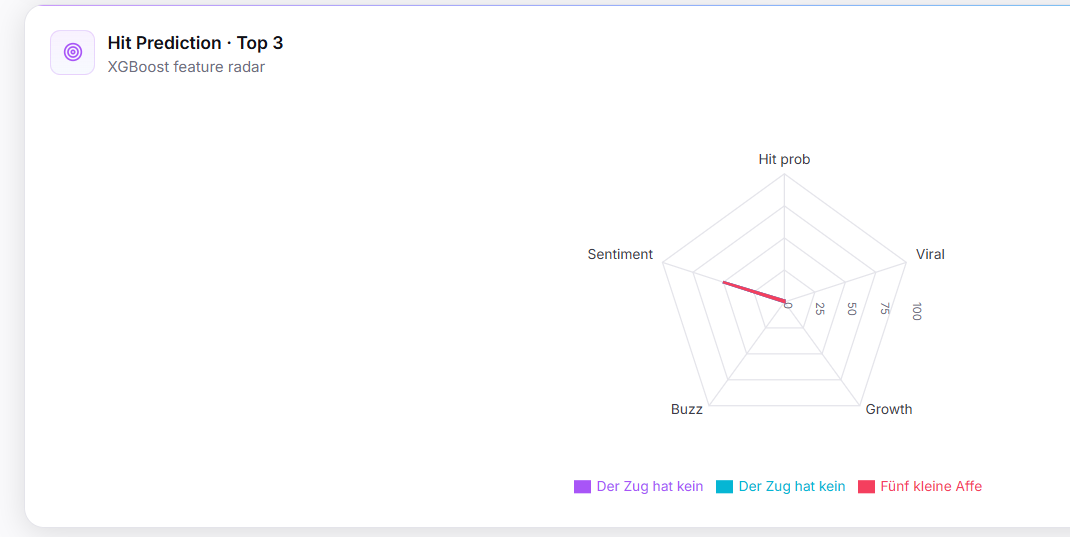
\includegraphics[width=\textwidth]{figures/visualize-hit.png}
    \caption{Hit Explanation: SHAP weights, Radar 5 trục, Gemini narrative, Risk tier và Action suggestions}
    \label{fig:hit_explanation}
\end{figure}

\section{AI Chat (ReAct Agent)}

\subsection{Kiến trúc ReAct Agent}

AI Chat sử dụng kiến trúc \textbf{ReAct (Reasoning + Acting)} với \textbf{Gemini 3.1 Flash-Lite}. Thay vì chỉ trả lời dựa trên kiến thức có sẵn, mô hình được cấp quyền tự quyết định việc sử dụng công cụ để thu thập thông tin theo thời gian thực. Quy trình hoạt động của Agent tuân theo vòng lặp 4 bước:
\begin{enumerate}[leftmargin=*]
    \item \textbf{Thought (Suy nghĩ):} Phân tích yêu cầu và lên kế hoạch (ví dụ: ``Người dùng hỏi tại sao bài APT viral, mình cần tìm kiếm tin tức về bài APT trên Google...'').
    \item \textbf{Action (Hành động):} Lựa chọn và thực thi một công cụ phù hợp từ bộ công cụ (như \texttt{web\_search}, \texttt{get\_reddit\_buzz}).
    \item \textbf{Observation (Quan sát):} Phân tích dữ liệu thực tế do công cụ trả về.
    \item \textbf{Evaluate (Đánh giá):} Lặp lại chu trình nếu thông tin chưa đủ, hoặc đưa ra \textbf{Final Answer} (câu trả lời cuối cùng) nếu đã giải quyết xong.
\end{enumerate}

Sơ đồ vòng lặp ReAct được mô tả chi tiết ở Hình~\ref{fig:react_loop}.

\begin{figure}[H]
    \centering
    \resizebox{0.8\textwidth}{!}{
    \begin{tikzpicture}[
        node distance = 1.2cm and 1.5cm,
        box/.style = {draw, rectangle, rounded corners=5pt, minimum width=3.0cm, minimum height=1.2cm, align=center, font=\small\bfseries, line width=1pt},
        agent/.style = {box, fill=mprimary!10, draw=mprimary},
        thought/.style = {box, fill=maccent!10, draw=maccent},
        action/.style = {box, fill=borderblue!10, draw=borderblue},
        obs/.style = {box, fill=mgood!10, draw=mgood},
        final/.style = {box, fill=black!8, draw=black!60, dashed},
        arrow/.style = {draw=black!70, -{Stealth[scale=1.1]}, line width=1.1pt}
    ]

        \node (user) [agent, rounded corners=15pt] {Người dùng\\(Prompt)};
        \node (thought) [thought, below=of user] {1. Thought\\(Suy luận ngữ cảnh)};
        \node (action) [action, right=of thought] {2. Action\\(Gọi API / Tool)};
        \node (obs) [obs, right=of user] {3. Observation\\(Nhận kết quả)};
        
        \node (final) [final, left=of thought] {Final Answer\\(Trả lời user)};

        \draw [arrow] (user) -- (thought);
        \draw [arrow] (thought) -- (action);
        \draw [arrow] (action) -- node[right] {Thực thi} (obs);
        \draw [arrow] (obs) -- node[above] {Phân tích} (user);
        
        \draw [arrow] (thought) -- node[above] {Đủ thông tin} (final);
        
        % Vòng lặp
        \draw[arrow, maccent, dashed] (obs.north) |- ++(0, 0.8) -| node[pos=0.25, above, text=maccent] {Vòng lặp (Max 6 Iterations)} (user.north);

    \end{tikzpicture}
    }
    \caption{Kiến trúc vòng lặp ReAct (Reasoning + Acting) của AI Agent}
    \label{fig:react_loop}
\end{figure}

Agent giới hạn \textbf{tối đa 6 vòng lặp} (MAX\_ITERATIONS=6) nhằm tránh tình trạng suy luận vô hạn (infinite loop) tốn chi phí API. Mỗi thao tác được stream real-time đến frontend qua giao thức \textbf{SSE (Server-Sent Events)}.

\subsection{Bộ công cụ (Tool Registry)}

Agent có 8 công cụ:

\begin{table}[H]
\centering
\caption{Bộ công cụ của ReAct Agent}
\label{tab:tools}
\begin{tabular}{|l|l|}
\hline
\textbf{Tool} & \textbf{Mô tả} \\
\hline
\texttt{web\_search} & DuckDuckGo web search (hỗ trợ region='vi-vn' cho kết quả VN) \\
\texttt{web\_news} & DuckDuckGo news search \\
\texttt{get\_global\_charts} & Top tracks toàn cầu từ Last.fm \\
\texttt{get\_country\_top} & Top tracks theo quốc gia \\
\texttt{get\_tiktok\_trends} & TikTok viral từ Deezer \\
\texttt{get\_reddit\_buzz} & Hot posts + sentiment từ subreddit \\
\texttt{get\_youtube\_for\_track} & Tìm MV YouTube + stats \\
\texttt{viral\_score} & Tính viral score 0-100 cho 1 bài \\
\hline
\end{tabular}
\end{table}

\subsection{Tính năng Graceful Fallback}

Điểm vượt trội của hệ thống là khả năng \textbf{tự phục hồi (Self-Healing)} khi gặp sự cố, đảm bảo tính liên tục của trải nghiệm người dùng:
\begin{itemize}[leftmargin=*]
    \item \textbf{Tool Failure Recovery:} Khi một công cụ gặp lỗi (ví dụ: DuckDuckGo bị chặn rate limit hoặc timeout), agent không làm sập (crash) toàn bộ phiên chat. Thay vào đó, nó tạo ra một ``Observation'' chứa thông báo lỗi, từ đó ``Thought'' tiếp theo sẽ chủ động chuyển sang sử dụng công cụ khác hoặc dùng kiến thức nội tại (internal knowledge) để trả lời. Đây là kỹ thuật \textit{graceful degradation} rất quan trọng cho các hệ thống production.
    \item \textbf{Local Context (Ưu tiên ngữ cảnh Việt Nam):} Bảng xếp hạng của Last.fm tại Việt Nam thường thiếu dữ liệu hoặc bị lỗi thời. Để khắc phục, System Prompt được thiết kế đặc biệt: buộc agent \textbf{ưu tiên dùng công cụ web\_search (region='vi-vn')} khi phát hiện từ khoá V-Pop. Do đó, Agent sẽ trích xuất số liệu trực tiếp từ Zing MP3, NhacCuaTui, hoặc Spotify VN thay vì phụ thuộc cứng vào Last.fm. Đây cũng là lý do tính năng AI Insights luôn cho kết quả đánh giá thị hiếu Việt Nam rất chuẩn xác dù dữ liệu World Map có thể bị nhiễu.
\end{itemize}

\begin{figure}[H]
    \centering
    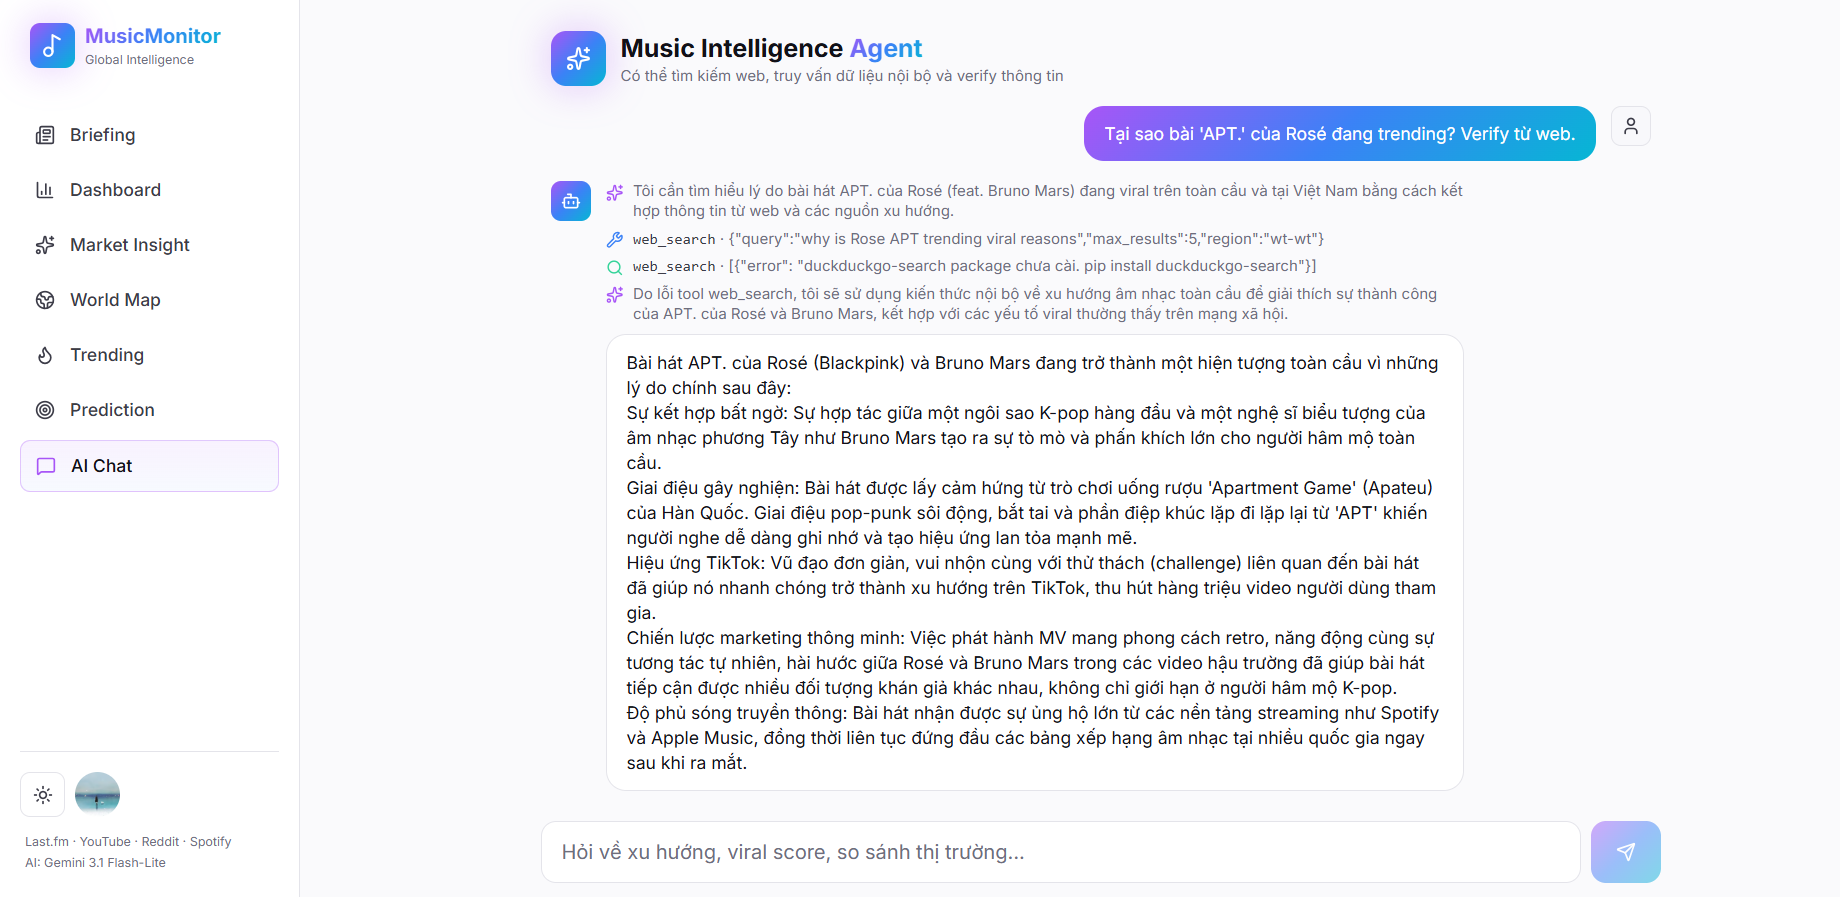
\includegraphics[width=\textwidth]{figures/ai-chat.png}
    \caption{AI Chat: ReAct loop với Thought, Action và Observation, tự phục hồi khi tool lỗi}
    \label{fig:ai_chat}
\end{figure}

% ============================================================
% CHƯƠNG 6 — BẢO MẬT VÀ TRIỂN KHAI
% ============================================================
\chapter{BẢO MẬT VÀ TRIỂN KHAI}

\section{Xác thực và Phân quyền (Clerk)}

Hệ thống dùng \textbf{Clerk} làm Identity Platform để quản lý xác thực:
\begin{itemize}
    \item \textbf{SSO:} Đăng nhập qua Google hoặc Email/Password.
    \item \textbf{Middleware bảo vệ:} \texttt{auth().protect()} chặn truy cập trái phép vào dashboard, AI Chat, Data Pipeline.
    \item \textbf{Session management:} Clerk tự quản lý JWT token, refresh token, connected accounts.
    \item \textbf{Future RBAC:} Nền móng sẵn sàng cho phân quyền Admin/Viewer.
\end{itemize}

Route \texttt{/} và \texttt{/sign-in} là public; mọi route dashboard đều protected.

Sơ đồ luồng xác thực và phân quyền được trình bày ở Hình~\ref{fig:auth_flow}.

\begin{figure}[H]
    \centering
    \resizebox{0.85\textwidth}{!}{
    \begin{tikzpicture}[
        node distance = 0.8cm and 1.5cm,
        box/.style = {draw, rectangle, rounded corners=5pt, minimum width=2.8cm, minimum height=1.0cm, align=center, font=\small\bfseries, line width=1pt},
        decision/.style = {draw, diamond, aspect=2.2, minimum width=3.0cm, minimum height=0.9cm, align=center, font=\small\bfseries, line width=1pt, fill=maccent!10, draw=maccent},
        userbox/.style = {box, fill=mprimary!8, draw=mprimary},
        process/.style = {box, fill=borderblue!6, draw=borderblue},
        result/.style = {box, fill=mgood!10, draw=mgood},
        reject/.style = {box, fill=red!8, draw=red!60},
        arrow/.style = {draw=black!70, -{Stealth[scale=1.1]}, line width=1.1pt}
    ]

        \node (user) [userbox] {Người dùng\\truy cập route};
        \node (middleware) [process, below=of user] {Clerk Middleware\\(Next.js)};
        \node (check) [decision, below=0.8cm of middleware] {Route\\protected?};
        \node (public) [result, left=2.0cm of check] {Cho phép truy cập\\(Public page)};
        \node (hasToken) [decision, right=2.0cm of check] {Có JWT\\token?};
        \node (verify) [process, below=0.8cm of hasToken] {Xác thực JWT\\(Clerk verify)};
        \node (redirect) [reject, above=0.6cm of hasToken] {Redirect\\→ /sign-in};
        \node (granted) [result, below=0.8cm of verify] {Truy cập\\Dashboard};

        \draw [arrow] (user) -- (middleware);
        \draw [arrow] (middleware) -- (check);
        \draw [arrow] (check) -- node[above, font=\footnotesize\bfseries] {Không} (public);
        \draw [arrow] (check) -- node[above, font=\footnotesize\bfseries] {Có} (hasToken);
        \draw [arrow] (hasToken) -- node[left, font=\footnotesize\bfseries] {Không} (redirect);
        \draw [arrow] (hasToken) -- node[left, font=\footnotesize\bfseries] {Có} (verify);
        \draw [arrow] (verify) -- (granted);

    \end{tikzpicture}
    }
    \caption{Luồng xác thực và phân quyền: Clerk Middleware kiểm tra JWT cho mọi protected route}
    \label{fig:auth_flow}
\end{figure}

\begin{figure}[H]
    \centering
    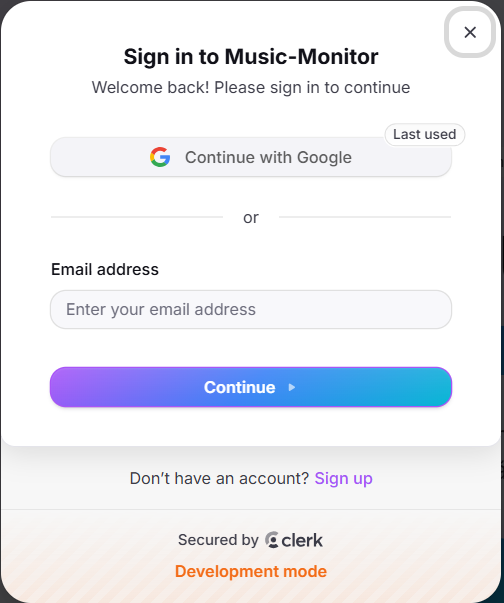
\includegraphics[width=0.5\textwidth]{figures/sign-in.png}
    \caption{Trang đăng nhập với SSO (Google/Email) qua Clerk}
    \label{fig:signin}
\end{figure}

\begin{figure}[H]
    \centering
    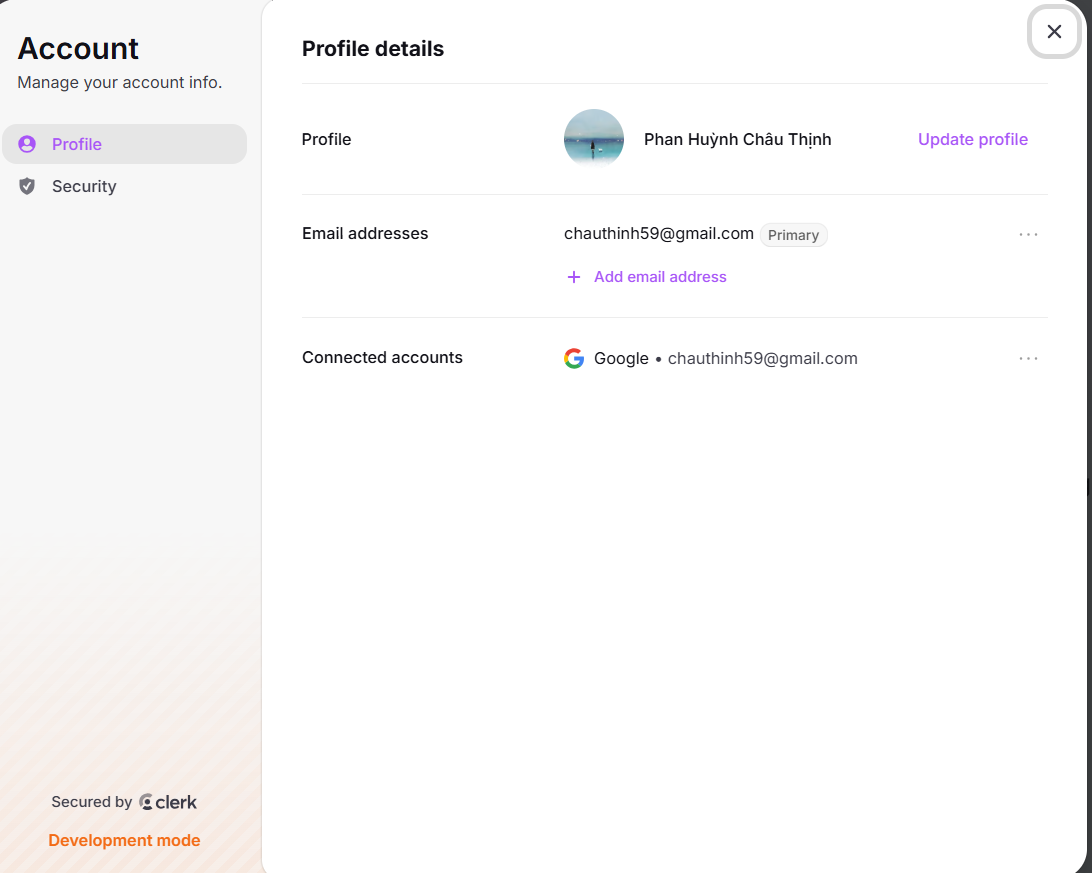
\includegraphics[width=0.5\textwidth]{figures/clerk-profile.png}
    \caption{Giao diện quản lý hồ sơ và bảo mật tài khoản cung cấp bởi Clerk}
    \label{fig:clerk_profile}
\end{figure}

\section{Xử lý Lỗi và Graceful Degradation}

Hệ thống được thiết kế với triết lý \textbf{``không bao giờ crash toàn bộ''} - khi một thành phần gặp sự cố, hệ thống tự động chuyển sang phương án dự phòng thay vì hiển thị lỗi cho người dùng. Các chiến lược chính:

\begin{itemize}
    \item \textbf{YouTube API hết quota (HTTP 403):} Tự động fallback sang Last.fm playcount làm chỉ số thay thế cho view count. Dashboard vẫn hiển thị đầy đủ dữ liệu.
    \item \textbf{Firebase credentials lỗi hoặc không khả dụng:} Backend tự động chuyển sang \texttt{\_MemDB} (in-memory dictionary) - hệ thống vẫn hoạt động bình thường trong phiên demo, chỉ mất persistence khi restart.
    \item \textbf{Gemini AI quota/timeout:} Trả về bản tin dự phòng (\texttt{\_fallback\_briefing()}) được tạo từ dữ liệu thô, đảm bảo Daily Briefing luôn có nội dung.
    \item \textbf{Song song hoá an toàn:} Tất cả các lệnh gọi API song song đều sử dụng \texttt{asyncio.gather(\allowbreak{}return\_exceptions=True)} - nếu 1 trong 4 nguồn lỗi, 3 nguồn còn lại vẫn trả kết quả bình thường thay vì crash toàn bộ request.
    \item \textbf{ReAct Agent tự phục hồi:} Khi một tool (ví dụ: DuckDuckGo) không khả dụng, agent nhận observation lỗi và tự chuyển sang tool khác hoặc dùng kiến thức nội bộ để trả lời - không crash hội thoại.
    \item \textbf{Deezer strict mode:} Khi thu thập chart cho World Map, hệ thống chỉ lấy chart thực của quốc gia (\texttt{strict=True}), không fallback global chart để tránh nhiễu dữ liệu clustering.
\end{itemize}

\section{Quản lý API Key và Môi trường}

Tất cả secret keys được quản lý qua file \texttt{.env} (không commit lên git). Cấu hình dùng \textbf{pydantic-settings} để validate:

Sơ đồ cơ chế quản lý và xác thực biến môi trường (Environment Variables) được mô tả ở Hình~\ref{fig:pydantic_settings}.

\begin{figure}[H]
    \centering
    \resizebox{0.95\textwidth}{!}{
    \begin{tikzpicture}[
        node distance = 1.0cm and 3.0cm,
        shadow/.style={preaction={fill=black, opacity=0.15, transform canvas={xshift=3pt, yshift=-3pt}}},
        box/.style = {draw, rectangle, rounded corners=6pt, align=center, line width=1.2pt, shadow, inner sep=12pt},
        envbox/.style = {box, fill=black!3, draw=black!40, minimum width=4.5cm, minimum height=4.0cm, font=\small\ttfamily, align=left},
        process/.style = {box, fill=borderblue!8, draw=borderblue, minimum width=4.0cm, minimum height=2.0cm, font=\small\bfseries\sffamily},
        validbox/.style = {box, fill=mgood!6, draw=mgood, minimum width=4.5cm, minimum height=4.0cm, font=\small\ttfamily, align=left},
        arrow/.style = {draw=black!50, -{Stealth[scale=1.2]}, line width=1.5pt}
    ]

        % .env File
        \node (env) [envbox] {
            \underline{\textbf{File .env (Raw String)}}\\[0.3cm]
            GEMINI\_API\_KEY=...\\
            FIREBASE\_CERT\_PATH=...\\
            LASTFM\_API\_KEY=...\\
            YOUTUBE\_API\_KEY=...\\
            REDDIT\_USER\_AGENT=...\\
            SPOTIFY\_CLIENT\_ID=...\\
            SPOTIFY\_CLIENT\_SECRET=...
        };
        
        % Pydantic Engine
        \node (engine) [process, right=of env] {pydantic-settings\\[0.15cm](BaseSettings)};
        
        % Validated Settings
        \node (settings) [validbox, right=of engine] {
            \underline{\textbf{Settings Instance (Validated)}}\\[0.3cm]
            gemini\_api\_key: \textcolor{borderblue}{str}\\
            firebase\_cert\_path: \textcolor{borderblue}{str}\\
            lastfm\_api\_key: \textcolor{borderblue}{str}\\
            youtube\_api\_key: \textcolor{borderblue}{str}\\
            reddit\_user\_agent: \textcolor{borderblue}{str}\\
            spotify\_client\_id: \textcolor{borderblue}{str}\\
            spotify\_client\_secret: \textcolor{borderblue}{str}
        };

        % Arrows
        \draw [arrow] (env) -- node[midway, above=0.15cm, font=\footnotesize\bfseries\sffamily, align=center, text=black!80] {Đọc tự động\\(Config.env\_file)} (engine);
        \draw [arrow] (engine) -- node[midway, above=0.15cm, font=\footnotesize\bfseries\sffamily, align=center, text=black!80] {Ép kiểu \&\\Báo lỗi nếu thiếu} (settings);

    \end{tikzpicture}
    }
    \caption{Cơ chế cấu hình và xác thực biến môi trường tự động bằng Pydantic}
    \label{fig:pydantic_settings}
\end{figure}

\section{Rate Limiting và Quota Management}

\textbf{Gemini Rate Limiter:} Free tier giới hạn 14 req/phút. Hệ thống implement rate limiter bằng asyncio queue, giới hạn 12 req/62s (an toàn hơn 14/phút). Exponential backoff khi gặp 429 (tối đa 3 lần retry). In-memory daily cache cho mọi AI insight.

\textbf{YouTube Quota:} 10.000 units/ngày. Batch fetch chỉ lấy top 8-10 tracks, tránh gọi quá nhiều.

\section{Triển khai}

\begin{itemize}
    \item \textbf{Frontend:} Vercel (Next.js 14, port 3000)
    \item \textbf{Backend:} Render.com (FastAPI + Uvicorn, port 8000)
    \item \textbf{Database:} Firebase Firestore (Google Cloud)
    \item \textbf{CI/CD:} Auto-deploy từ GitHub khi push lên main branch
\end{itemize}

CORS được cấu hình chặt chẽ: chỉ cho phép origin từ localhost (development) và domain Vercel (production).

% ============================================================
% CHƯƠNG 7 — KẾT LUẬN VÀ HƯỚNG PHÁT TRIỂN
% ============================================================
\chapter{KẾT LUẬN VÀ HƯỚNG PHÁT TRIỂN}

\section{Kết luận}

Dự án \textbf{World Music Intelligence Monitor} đã xây dựng thành công một nền tảng phân tích âm nhạc thông minh end-to-end, tích hợp đa nguồn dữ liệu và AI. Các kết quả đạt được:

\textbf{Thu thập và xử lý dữ liệu:} Pipeline đa nguồn (Last.fm, YouTube, Reddit, Deezer) hoạt động ổn định với cache 3 lớp, đảm bảo luôn có dữ liệu hiển thị dù API bị giới hạn. Decay factor xử lý bias tuổi MV cho kết quả hit prediction thực tế hơn.

\textbf{Phân tích và trực quan hoá:} Dashboard tổng hợp KPI, chart, anomaly alert và AI briefing trên cùng một màn hình. World Map phân cụm 89 quốc gia theo gu âm nhạc bằng K-Means + PCA. VADER NLP phân tích cảm xúc Reddit real-time.

\textbf{Machine Learning:} XGBoost hit predictor với ROC AUC = 1.0 trên dữ liệu synthetic. Pipeline tự động thu thập đặc trưng từ 4 nguồn, xử lý seasonality và genre popularity. Explainable AI với SHAP + Radar + Gemini narrative.

\textbf{AI Agent:} ReAct Agent tự gọi công cụ, tự phục hồi khi lỗi, streaming real-time qua SSE. Đặc biệt xử lý tốt câu hỏi về V-Pop bằng cách ưu tiên web\_search tiếng Việt thay vì Last.fm.

\textbf{Bài học rút ra:} Tích hợp AI thực sự không chỉ là gọi API - phải hiểu giới hạn của từng nguồn dữ liệu (Deezer VN, Last.fm quota, YouTube decay), thiết kế fallback thông minh và cache hợp lý để hệ thống vận hành ổn định trên free tier.

\section{Insight: Âm nhạc trên toàn cầu}

Trong số các phát hiện từ hệ thống, insight từ tính năng \textbf{World Map - K-Means Clustering} là ấn tượng nhất về mặt văn hoá và có chiều sâu phân tích cao nhất.

Khi thuật toán K-Means phân cụm 89 quốc gia dựa trên vector đặc trưng thể loại âm nhạc 16 chiều, kết quả thu được \textbf{hoàn toàn trái với kỳ vọng địa lý thông thường}: Các cụm âm nhạc không khớp với bản đồ châu lục, ngôn ngữ hay khoảng cách địa lý, mà khớp với \textbf{luồng văn hoá đại chúng toàn cầu}.

\begin{itemize}
    \item \textbf{Phát hiện cụ thể:} Cụm \textit{K-Pop dominant} không chỉ bao phủ Đông Á mà lan sang cả các quốc gia Đông Nam Á, một phần Trung Đông và thậm chí Mỹ Latin, phản ánh sức mạnh lan toả của Làn sóng Hàn Quốc (Hallyu). Tương tự, cụm \textit{Latin-dominant} mở rộng vượt ra ngoài Mỹ Latin để ôm trọn nhiều nước Đông Nam Á và một số quốc gia Châu Phi, nơi nhạc Reggaeton và Latin Pop đang âm thầm chiếm lĩnh thị trường nhờ TikTok.
    \item \textbf{Giải thích bằng dữ liệu (Data-driven Interpretation):} Đây không phải một sự trùng hợp ngẫu nhiên. Dữ liệu cho thấy streaming và mạng xã hội, đặc biệt là TikTok Viral và YouTube, đang hoạt động như một \textbf{``bộ san phẳng văn hoá'' (cultural equalizer)}: Một bài hát gây bão tại Seoul hay Bogotá có thể đồng thời leo thẳng lên Top 10 tại Jakarta hay Cairo chỉ sau vài ngày. Khoảng cách địa lý không còn là rào cản khuếch tán âm nhạc.
    \item \textbf{Giá trị thực tiễn:} Các nhãn hàng âm nhạc (Music Labels) và nền tảng streaming có thể dùng mô hình phân cụm này để \textbf{thiết kế chiến lược phân phối nội dung xuyên biên giới (cross-border content distribution)} chính xác hơn, thay vì marketing theo địa lý truyền thống. Ví dụ: khi phát hành một album K-Pop, thay vì chỉ target Châu Á, dữ liệu gợi ý nên đồng thời ưu tiên thị trường Mỹ Latin và Đông Nam Á vì chúng thuộc cùng một ``vùng văn hoá'' theo dữ liệu thực tế.
\end{itemize}

Insight này là bằng chứng rõ ràng nhất cho luận điểm trung tâm của hệ thống: \textit{Âm nhạc hiện đại không còn là sản phẩm của một vùng đất, mà là sản phẩm của những thuật toán gợi ý toàn cầu.}

\section{Hướng Phát Triển}

\textbf{1. Nâng quota API và tách worker:} Ưu tiên \#1 cho production thật. Tách scheduler thành worker riêng, dùng message queue (Redis/Celery). Nâng YouTube API key lên Billing để tăng quota.

\textbf{2. Event-driven streaming thật:} Hiện tại polling định kỳ. Chuyển sang event-driven với WebSocket/Kafka cho true real-time.

\textbf{3. Phân quyền RBAC:} Triển khai Admin/Viewer roles với Clerk. Admin có thể trigger manual refresh, xem metrics; Viewer chỉ đọc.

\textbf{4. Mô hình hit prediction với dữ liệu thực:} Sau 3-6 tháng thu thập, có thể retrain XGBoost với dữ liệu lịch sử thực từ Firestore thay vì dữ liệu synthetic.

\textbf{5. Tích hợp thêm TikTok API chính thức:} Khi có API key, thay thế Deezer TikTok proxy bằng dữ liệu TikTok trực tiếp để chính xác hơn.

% ============================================================
% TÀI LIỆU THAM KHẢO
% ============================================================
\begin{thebibliography}{99}

\bibitem{fastapi}
Ramírez, S. (2018-2026).
FastAPI Framework.
\textit{Available at:} \url{https://fastapi.tiangolo.com/}

\bibitem{nextjs}
Vercel (2016-2026).
Next.js Documentation.
\textit{Available at:} \url{https://nextjs.org/docs}

\bibitem{xgboost}
Chen, T., \& Guestrin, C. (2016).
XGBoost: A Scalable Tree Boosting System.
\textit{Proceedings of the 22nd ACM SIGKDD International Conference on Knowledge Discovery and Data Mining}.
\url{https://arxiv.org/abs/1603.02754}

\bibitem{kmeans}
MacQueen, J. (1967).
Some Methods for Classification and Analysis of Multivariate Observations.
\textit{Proceedings of the 5th Berkeley Symposium on Mathematical Statistics and Probability}, 1, 281-297.

\bibitem{vader}
Hutto, C., \& Gilbert, E. (2014).
VADER: A Parsimonious Rule-based Model for Sentiment Analysis of Social Media Text.
\textit{Proceedings of the 8th International AAAI Conference on Weblogs and Social Media}.

\bibitem{react_agent}
Yao, S., et al. (2023).
ReAct: Synergizing Reasoning and Acting in Language Models.
\textit{International Conference on Learning Representations (ICLR)}.
\url{https://arxiv.org/abs/2210.03629}

\bibitem{gemini}
Google DeepMind (2023-2026).
Gemini API Documentation.
\textit{Available at:} \url{https://ai.google.dev/}

\bibitem{firebase}
Google (2014-2026).
Firebase Firestore Documentation.
\textit{Available at:} \url{https://firebase.google.com/docs/firestore}

\bibitem{lastfm}
Last.fm (2002-2026).
Last.fm API Documentation.
\textit{Available at:} \url{https://www.last.fm/api}

\bibitem{deezer}
Deezer (2007-2026).
Deezer API Documentation.
\textit{Available at:} \url{https://developers.deezer.com/api}

\end{thebibliography}

% ============================================================
% PHỤ LỤC
% ============================================================
\appendix
\renewcommand{\appendixname}{Phụ lục}

\chapter{PHỤ LỤC}

\section{Liên kết dự án}
\begin{itemize}
    \item Source code: \href{https://github.com/Thinh59/Music-Monitor}{https://github.com/Thinh59/Music-Monitor}
    \item Video demo: \href{https://youtu.be/KjsEracAcn4?si=pUIJTtgdBZ43e7jL}{https://youtu.be/KjsEracAcn4}
    \item Kaggle notebook (EDA \& Training): \href{https://www.kaggle.com/}{music-monitor-eda-training.ipynb}
\end{itemize}

\section{Bảng API Endpoints}

\begin{longtable}{|l|l|p{6.5cm}|}
\hline
\textbf{Endpoint} & \textbf{Method} & \textbf{Mô tả} \\
\hline
\endfirsthead
\hline
\textbf{Endpoint} & \textbf{Method} & \textbf{Mô tả} \\
\hline
\endhead
\texttt{/api/charts/global} & GET & Top tracks toàn cầu (Last.fm) \\
\hline
\texttt{/api/charts/country/\{name\}} & GET & Top tracks theo quốc gia \\
\hline
\texttt{/api/trends/tiktok} & GET & TikTok viral list (Deezer) \\
\hline
\texttt{/api/trends/viral} & GET & Reddit hot posts + VADER sentiment \\
\hline
\texttt{/api/trends/overview} & GET & Tổng hợp 3 nguồn song song \\
\hline
\texttt{/api/trends/youtube/batch} & GET & YouTube stats cho top tracks \\
\hline
\texttt{/api/trends/spike/\{track\}} & GET & Viral score tổng hợp 0-100 \\
\hline
\texttt{/api/trends/explain/\{track\}} & GET & Gemini giải thích tại sao viral \\
\hline
\texttt{/api/map/clusters} & GET & Phân cụm 89 quốc gia (K-Means, cache file) \\
\hline
\texttt{/api/map/country/\{iso\}/top} & GET & Top tracks tại 1 quốc gia \\
\hline
\texttt{/api/map/country/\{iso\}/ai-insight} & GET & Gemini AI insight cho quốc gia \\
\hline
\texttt{/api/prediction/quick} & POST & Tự động thu thập data rồi predict \\
\hline
\texttt{/api/prediction/top-candidates} & GET & Top bài tiềm năng \\
\hline
\texttt{/api/briefing/daily} & GET & Daily AI Briefing (cache theo ngày) \\
\hline
\texttt{/api/analysis/distribution/genre} & GET & Phân phối genre từ top artists \\
\hline
\texttt{/api/analysis/insight/market-summary} & GET & Market Intelligence Summary \\
\hline
\texttt{/api/agent/chat} & POST & Stream SSE agent response (ReAct) \\
\hline
\end{longtable}

\section{Schema Firestore}

\begin{table}[H]
\centering
\caption{Cấu trúc các collections trong Firebase Firestore}
\label{tab:firestore_schema}
\begin{tabularx}{\textwidth}{|l|l|X|}
\hline
\textbf{Collection/Document} & \textbf{Cập nhật} & \textbf{Nội dung} \\
\hline
\texttt{cache/global\_top} & Mỗi 6h (scheduler) & Top 50 tracks toàn cầu Last.fm: track name, artist, playcount, listeners, updated\_at \\
\hline
\texttt{youtube\_snapshots/\{id\}/history} & On-demand & Lịch sử view count YouTube: timestamps, views, likes, comments \\
\hline
\end{tabularx}
\end{table}

\section{Cấu trúc thư mục dự án}

\begin{verbatim}
Music-Monitor/
├── backend/
│   ├── app/
│   │   ├── main.py              # FastAPI entrypoint
│   │   ├── config.py            # Pydantic Settings (.env)
│   │   ├── database.py          # Firebase Admin SDK
│   │   ├── scheduler.py         # APScheduler (polling 6h)
│   │   ├── routers/             # 7 API router modules
│   │   ├── services/            # 5 external API clients
│   │   ├── ai/                  # AI/ML modules + tools/
│   │   └── models/              # hit_predictor.joblib
│   └── requirements.txt
├── frontend/
│   ├── src/
│   │   ├── app/                 # Next.js 14 App Router pages
│   │   ├── components/          # React components + charts/
│   │   ├── lib/                 # API fetch + SSE client
│   │   └── types/               # TypeScript interfaces
│   └── package.json
├── kaggle/
│   └── music-monitor-eda-training.ipynb
├── report/                      # Báo cáo LaTeX
├── slides/                      # Slide thuyết trình
└── docker-compose.yml
\end{verbatim}

\end{document}